\documentclass[conference]{IEEEtran}
\IEEEoverridecommandlockouts
\usepackage[utf8]{inputenc}
\usepackage[english]{babel}
\usepackage{cite}
\usepackage{amsmath,amssymb,amsfonts}
\usepackage{algorithmic}
\usepackage{graphicx}
\usepackage{textcomp}
\usepackage{xcolor}
\usepackage{hyperref}
\usepackage{booktabs}
\usepackage{array}
\usepackage{multirow}
\usepackage{float}
\usepackage{tikz}
\usepackage{listings}
\usepackage{geometry}
\usepackage{tabularx}
\usepackage{longtable}
\usepackage{enumitem}
\usetikzlibrary{shapes.geometric, arrows.meta, positioning, calc, fit, backgrounds}

\geometry{
  letterpaper,
  top=2.5cm, bottom=2.5cm,
  left=2.5cm, right=2.5cm
}
\onecolumn

%% ---- Shared TikZ styles ----
\tikzset{
  block/.style  = {rectangle, draw, fill=blue!10,   text width=2.9cm,
                   text centered, rounded corners, minimum height=0.95cm, font=\small},
  blockG/.style = {rectangle, draw, fill=green!15,  text width=2.9cm,
                   text centered, rounded corners, minimum height=0.95cm, font=\small},
  blockO/.style = {rectangle, draw, fill=orange!15, text width=2.9cm,
                   text centered, rounded corners, minimum height=0.95cm, font=\small},
  blockR/.style = {rectangle, draw, fill=red!12,    text width=2.9cm,
                   text centered, rounded corners, minimum height=0.95cm, font=\small},
  blockP/.style = {rectangle, draw, fill=purple!12, text width=2.9cm,
                   text centered, rounded corners, minimum height=0.95cm, font=\small},
  blockY/.style = {rectangle, draw, fill=yellow!20, text width=2.9cm,
                   text centered, rounded corners, minimum height=0.95cm, font=\small},
  arrow/.style  = {thick, ->, >=Stealth},
  darrow/.style = {thick, <->, >=Stealth},
  dasharrow/.style = {thick, dashed, ->, >=Stealth},
}

\lstset{
  basicstyle=\ttfamily\footnotesize,
  breaklines=true,
  frame=single,
  commentstyle=\color{gray},
  keywordstyle=\color{blue},
  numbers=left,
  numberstyle=\tiny\color{gray},
  xleftmargin=1.5em,
  framexleftmargin=1.5em,
}

\begin{document}

%% ============================================================
%%  TITLE
%% ============================================================
\title{Distributed Cloud Architecture for Predictive Detection and\\
Mitigation of Computer Vision Syndrome through Behavioral Analytics:\\
General Architecture and Prototype Design}

\author{
  \IEEEauthorblockN{Andersson David Sánchez Méndez,
                    Cristian Santiago Pedraza Rodríguez,
                    Jeisson David Sánchez Gómez}
  \IEEEauthorblockA{Systems Engineering Program\\
    Escuela Colombiana de Ingeniería Julio Garavito, Bogotá D.C., Colombia\\
    \{andersson.sanchez-m, cristian.pedraza-r, jeisson.sanchez-g\}@mail.escuelaing.edu.co}
}

\maketitle

%% ============================================================
%%  ABSTRACT
%% ============================================================
\begin{abstract}
Computer Vision Syndrome (CVS), also known as Digital Eye Strain (DES), is a critical
occupational health challenge affecting approximately 69\% of the global population
\cite{b15} and generating an estimated \$151 billion in combined productivity losses,
direct healthcare costs, and well-being impacts in the United States alone during 2023
\cite{b16}. Despite growing awareness in both clinical and enterprise environments,
existing mitigation tools remain fundamentally reactive, isolated at the device level,
and architecturally incapable of supporting population-level analysis or proactive risk
management at organizational scale. This article presents the complete general software
architecture and the prototype-level design of a distributed, cloud-native platform for
the continuous ingestion, processing, and machine-learning-based analysis of biometric
and behavioral telemetry collected from edge devices. Building on the state-of-the-art
analysis published in the first phase of this project, we formalize a four-layer
architecture comprising an Edge Ingestion Layer, a Cloud Messaging Layer, an
Asynchronous Processing and Persistence Layer, and a Machine Learning Inference Layer.
Each layer is described through complementary architectural views aligned with the
IEEE/ISO~42010 standard: context, component, data-flow, deployment, and security.
The prototype is realized as a set of containerized microservices orchestrated with
Kubernetes, a Kafka-based streaming pipeline, an InfluxDB time-series data store, and
an XGBoost gradient-boosted CVS Risk Score inference module. We additionally present
the alignment of the platform with the TOGAF Enterprise Architecture framework,
formalize five Architecture Decision Records (ADRs), document the applied microservices
design patterns (Circuit Breaker, CQRS, Database-per-Service, and Event Sourcing), and
detail the CI/CD, observability, and data governance sub-architectures. Target Service
Level Objectives for availability, scalability, security, and ML accuracy are defined
and the evaluation methodology for the third project phase is specified.
\end{abstract}

\begin{IEEEkeywords}
Computer Vision Syndrome, Distributed Architecture, Cloud Native, Apache Kafka,
Kubernetes, InfluxDB, Machine Learning, Microservices, IoT Telemetry, Federated Privacy,
Enterprise Architecture, TOGAF, CQRS, Circuit Breaker, DevSecOps, Behavioral Analytics.
\end{IEEEkeywords}

%% ============================================================
\section{Introduction}
%% ============================================================

The post-pandemic reconfiguration of knowledge work has produced an unprecedented
intensification of digital screen exposure across the global workforce. Recent longitudinal
surveys indicate that knowledge workers now accumulate, on average, 99.2 hours of screen
time per week, with weekday exposure alone representing approximately 93\% of waking
hours \cite{b17}. These figures are not confined to a single geography or labor sector:
a 2024 meta-analysis synthesizing data from 103 cross-sectional studies encompassing
66,577 participants determined that the pooled global prevalence of Computer Vision
Syndrome (CVS) stands at approximately 69\% of the working population \cite{b15}.
The direct occupational consequence is substantial: 71\% of affected desk workers report
measurable productivity impacts attributable to CVS, with a mean productivity reduction
of 18.6\%---equivalent to roughly 7.4 lost productive hours per working week
\cite{b17}. In aggregate, unmanaged CVS-related screen exposure incurred \$50.6 billion
in productivity losses and over \$1.2 billion in direct healthcare system costs across
the United States in 2023 \cite{b16}.

From a software-engineering perspective, the root of the problem is not the absence of
detection hardware. Modern smartphones are already equipped with proximity sensors,
ambient light sensors, accelerometers, and high-resolution front-facing cameras.
The fundamental barrier is the \textbf{architectural inability} of current solutions
to move beyond device-level information silos. Tools such as \textit{Apple Screen Time},
\textit{Google Digital Wellbeing}, or \textit{f.lux} operate as closed-loop, reactive
systems: they collect data locally, apply static usage thresholds, and generate local
notifications, but they are structurally incapable of aggregating behavioral signals
across users to build predictive population-level models. This architectural fragmentation
prevents organizations from quantifying the ``digital wear'' of their human capital or
from implementing evidence-based proactive interventions at the departmental or
enterprise level.

The first phase of this research (State of the Art, First Tercio) established three
foundational scientific challenges that any viable architecture must address: (i)~energy-
efficient edge sensing, (ii)~behavioral data privacy and regulatory compliance, and
(iii)~elastic cloud scalability. It also introduced a four-layer architectural sketch.
The present article advances those foundational contributions substantially. Its specific
objectives are:
\begin{enumerate}
  \item To formally specify the \textbf{general architecture} of the CVS mitigation
        platform through five complementary architectural views: context, component,
        data-flow, deployment, and security.
  \item To present the \textbf{TOGAF-aligned enterprise architecture} view, mapping the
        four TOGAF domains (Business, Data, Application, Technology) to the platform's
        structural components.
  \item To detail the \textbf{prototype architecture} through concrete technology stack
        selections, Avro data schemas, Kafka topic designs, InfluxDB data models,
        REST API contracts, and ML pipeline specifications, formally documented as
        Architecture Decision Records (ADRs).
  \item To document the \textbf{applied microservices design patterns} that increase
        the platform's resilience, consistency, and observability.
  \item To specify the \textbf{CI/CD pipeline, observability stack, and data governance
        framework} that together constitute the operational architecture of the prototype.
  \item To define \textbf{target quality attributes} and Service Level Objectives (SLOs)
        that will be evaluated empirically in the third and final project phase.
\end{enumerate}

The remainder of the article is organized as follows.
Section~II provides the problem characterization and architectural scope.
Section~III presents an extended related work analysis.
Section~IV introduces the TOGAF Enterprise Architecture alignment.
Section~V presents the General Architecture through five views.
Section~VI describes the Prototype Architecture in full technical detail.
Section~VII documents the applied microservices design patterns.
Section~VIII details the CI/CD pipeline and DevOps architecture.
Section~IX presents the observability and monitoring architecture.
Section~X covers the data governance and compliance framework.
Section~XI formalizes the Architecture Decision Records.
Section~XII discusses quality attributes and SLOs.
Section~XIII presents an economic impact analysis.
Section~XIV covers the risk analysis and mitigation strategies.
Section~XV outlines the evaluation methodology for the third phase.
Section~XVI concludes the article.

%% ============================================================
\section{Problem Characterization and Architectural Scope}
%% ============================================================

\subsection{Clinical and Occupational Context}

CVS encompasses a range of ocular and musculoskeletal symptoms that manifest from
sustained digital screen interaction. Physiologically, the primary trigger is a
reduction in the spontaneous blink rate from a neurological baseline of 15--20 blinks
per minute to as few as 4--6 blinks per minute during active cognitive screen use
\cite{b2}. Reduced blinking disrupts the stability of the precorneal tear film, leading
to dry eye, asthenopia (eye fatigue), blurred vision, and accommodative dysfunction.
Compounding risk factors include screen-to-eye distances below 30~cm, mismatches between
ambient illuminance and screen brightness (measured in lux), and high-cognitive-load tasks
that further suppress blink frequency \cite{b3,b18}.

A 2024 controlled study demonstrated that CVS symptom severity scores begin to worsen
measurably from baseline as early as 10~minutes into continuous screen use, and that the
effect magnitude is significantly amplified under higher cognitive load conditions
\cite{b18}. This temporal granularity has a direct architectural implication: any
effective monitoring system must collect data \emph{continuously} at sub-minute intervals
rather than at the session level.

\subsection{Architectural Gap Analysis}

Table~\ref{tab:gap} summarizes the principal architectural gaps identified across the
three solution categories reviewed in the first phase of this project. Each row also
identifies the specific response this architecture provides to the identified gap.

\begin{table}[H]
  \centering
  \caption{Architectural Gap Analysis of Existing CVS Mitigation Approaches}
  \label{tab:gap}
  \begin{tabularx}{\textwidth}{>{\bfseries}p{3cm} p{4.5cm} p{4.5cm} p{3.2cm}}
    \toprule
    \textbf{Category} & \textbf{Representative Tools} &
    \textbf{Core Limitation} & \textbf{Gap Addressed Here} \\
    \midrule
    Edge-Only Well-being & Apple Screen Time, Google Digital Wellbeing, f.lux &
      No cross-device learning; static thresholds; no population baselines \cite{b1} &
      Federated ML; population risk profiling; organizational dashboards \\
    \addlinespace
    CV-Based Detection & CNN blink-rate monitors via webcam &
      High compute cost; privacy rejection due to continuous video recording;
      not viable as background service \cite{b4} &
      Non-visual proxy telemetry: ambient light, proximity, interaction time \\
    \addlinespace
    Healthcare IoT & Fog-computing cardiac monitors \cite{b5} &
      Not generalized to visual ergonomics; no enterprise EA alignment &
      SOA on cloud; TOGAF-aligned four-domain architecture; compliance layer \\
    \bottomrule
  \end{tabularx}
\end{table}

\subsection{System Boundary and Stakeholders}

The system boundary encompasses five principal actor categories:

\begin{itemize}
  \item \textbf{End User (Knowledge Worker):} installs the mobile agent; provides
        explicit informed consent; receives break-reminder push notifications.
  \item \textbf{Organizational Health Officer (OHO):} accesses aggregated, anonymized
        risk dashboards for workforce-level intervention planning and occupational
        health reporting.
  \item \textbf{IT / DevOps Administrator:} manages Kubernetes cluster health,
        CI/CD pipeline configuration, and cloud infrastructure provisioning.
  \item \textbf{ML Engineer:} curates anonymized training datasets, monitors model
        performance drift, and triggers retraining pipelines.
  \item \textbf{Regulatory / Compliance Officer:} audits GDPR compliance, data
        retention policies, and differential privacy configurations throughout
        the data lifecycle.
\end{itemize}

%% ============================================================
\section{Extended Related Work}
%% ============================================================

\subsection{Clinical Epidemiology of Digital Eye Strain}

The clinical literature on CVS has grown substantially since the early 2000s. Blehm
et al.\ \cite{b3} provided a seminal review covering the biomechanical mechanisms of
asthenopia, establishing the 30~cm minimum screen-to-eye distance and the role of ambient
lux mismatch as ergonomic thresholds. Sheppard and Wolffsohn \cite{b2} updated these
findings with a 2018 systematic review reporting CVS prevalence between 50\% and 90\%
among computer users, and quantifying the blink-rate reduction from 15--20 to 4--6
blinks per minute as the primary pathophysiological driver. More recently, Talens-Estarelles
et al.\ \cite{b18} provided controlled experimental evidence that CVS symptoms become
clinically significant within 10~minutes of continuous screen use and are strongly
modulated by cognitive load. This convergent body of evidence justifies the continuous,
30-second sampling interval adopted in our edge agent design, as opposed to session-level
aggregation strategies used by commercial tools.

\subsection{Non-Visual Proxy Sensing for Fatigue Detection}

The use of non-visual behavioral signals as proxies for fatigue states has been
explored extensively in the mobile sensing literature. Lane et al.\ \cite{b4} provided
a foundational survey of mobile phone sensing capabilities, demonstrating that
accelerometers, proximity sensors, and ambient light sensors collectively encode rich
behavioral context even without camera access. This work is directly relevant to our
architecture's choice to rely exclusively on non-visual telemetry, avoiding the
documented privacy rejection rates associated with continuous camera operation.

More recently, Alshurafa et al.\ \cite{b19} demonstrated the viability of wearable
sensor networks for multi-level fatigue prediction in manufacturing workers, achieving
competitive F1-scores using gradient-boosted tree classifiers on tabular biometric
features rather than deep neural networks. Their finding that lightweight tree ensembles
outperform neural networks on small-feature tabular datasets directly motivates our
choice of XGBoost for the CVS Risk Score model. Chae et al.\ \cite{b22} extended this
paradigm to visual fatigue specifically, demonstrating that classification models based
on physiological responses to office lighting conditions can accurately predict visual
fatigue onset, supporting the inclusion of ambient lux as a primary telemetry signal.

\subsection{Cloud and Fog Computing for Healthcare IoT}

Mutlag et al.\ \cite{b5} demonstrated how Fog Computing combined with microservices
can reduce end-to-end latency for critical cardiac telemetry to clinically acceptable
levels, and identified the architectural tradeoffs between edge-local and cloud-central
processing. Their work introduced the concept of heterogeneous computational tiers---
edge, fog, and cloud---that directly influenced our Layer~1 (edge buffering) and
Layer~2 (cloud gateway) design.

Mahmoud et al.\ \cite{b6} provided a 2024 survey of IoT application architectures,
classifying existing platforms along the dimensions of data flow, computational tier,
and communication protocol. Their analysis confirms that the \textit{publish-subscribe}
message-broker pattern (exemplified by Kafka) outperforms both polling and
synchronous REST for high-throughput IoT ingestion workloads, while providing
the decoupling necessary for independent scalability of producer and consumer components.

\subsection{Privacy-Preserving Machine Learning in Healthcare}

Berneker et al.\ \cite{b13} conducted a scoping review of federated machine learning
as a privacy-enhancing technology in medical research, mapping its compatibility with
European data protection law. Their analysis determined that federated learning---where
model training occurs locally on each institution's data without raw data
centralization---satisfies GDPR requirements under the data minimization and purpose
limitation principles. Ali et al.\ \cite{b14} extended this analysis to the IoT
healthcare context, presenting architectural patterns for federated learning integration
in smart healthcare platforms. Both works substantiate our ADR-004 designation of
federated learning as the long-term evolution path for the model training pipeline.

Alotaibi et al.\ \cite{b11} formalized the use of differential privacy with privacy
budget $\varepsilon \approx 1.0$ in real-time healthcare AI systems, demonstrating
that this configuration satisfies GDPR requirements while maintaining statistical utility
losses below 5 percentage points relative to unperturbed data. Mutlag et al.\ \cite{b23}
confirmed these findings in the context of federated learning for healthcare, providing
the mathematical framework for the Laplace noise mechanism we implement in the
Anonymizer Microservice.

\subsection{Time-Series Databases for IoT Telemetry}

The choice between specialized time-series databases for high-throughput IoT telemetry
has been a subject of active benchmarking. Comparative analyses \cite{b7} consistently
demonstrate that InfluxDB outperforms TimescaleDB on pure write-heavy IoT ingestion
workloads where queries are predominantly time-range aggregations, due to its purpose-built
line protocol and native compaction strategies optimized for monotonically increasing
timestamps. TimescaleDB retains advantages when workloads require complex relational
JOIN operations with non-time-series data. Our platform's write-dominant, aggregation-
focused access pattern---collecting three sensor readings every 30~seconds per device
across thousands of endpoints---aligns squarely with InfluxDB's performance advantage
profile.

\subsection{Kubernetes for Healthcare Platform Orchestration}

Boda and Allam \cite{b20} provided empirical evidence from production healthcare
deployments of Kubernetes-orchestrated microservices, documenting improvements in
resource utilization efficiency and system availability relative to VM-based deployments.
Their findings are particularly relevant to the Horizontal Pod Autoscaler (HPA)
configuration in our platform: they observed that setting CPU utilization targets
between 60\% and 70\% provides the best tradeoff between cost efficiency and
scale-out responsiveness, consistent with the 60\% and 70\% thresholds specified in
our prototype's Helm values.

%% ============================================================
\section{Enterprise Architecture Framework Alignment}
%% ============================================================

\subsection{TOGAF ADM Mapping}

The Open Group Architecture Framework (TOGAF) provides a globally recognized methodology
for designing, implementing, and governing enterprise IT architecture through its
Architecture Development Method (ADM) \cite{b24}. The ADM consists of a preliminary
phase and eight iterative development phases (A through H), covering architecture vision,
business architecture, information systems architecture, technology architecture,
opportunities and solutions, migration planning, implementation governance, and change
management. TOGAF has been adopted by 80\% of Global~50 companies and 60\% of
Fortune~500 companies, and its application to complex healthcare IoT systems has been
validated in multiple academic case studies \cite{b25}.

Table~\ref{tab:togaf} maps the CVS platform's development activities to the corresponding
TOGAF ADM phases, demonstrating formal alignment with enterprise architecture best practice.

\begin{table}[H]
  \centering
  \caption{TOGAF ADM Phase Mapping for the CVS Mitigation Platform}
  \label{tab:togaf}
  \begin{tabularx}{\textwidth}{p{3cm} p{4cm} X}
    \toprule
    \textbf{TOGAF ADM Phase} & \textbf{Primary Output} & \textbf{CVS Platform Artifact} \\
    \midrule
    Preliminary & Architecture principles; governance model &
      Stakeholder map; system boundary definition \\
    A: Architecture Vision & Stakeholder requirements; high-level solution concept &
      Problem characterization; four-layer sketch (First Tercio article) \\
    B: Business Architecture & Business capability model; organizational context &
      OHO intervention workflow; consent management process \\
    C: Information Systems & Data and application architecture &
      InfluxDB schema; Kafka topic design; REST API specification \\
    D: Technology Architecture & Technology stack; deployment topology &
      Kubernetes deployment view; Helm chart; Istio service mesh config \\
    E: Opportunities \& Solutions & Implementation roadmap; prototype identification &
      Prototype technology stack selection; ADR formalization \\
    F: Migration Planning & Prioritized implementation plan &
      Phase 2 (current) $\rightarrow$ Phase 3 evaluation roadmap \\
    G: Implementation Governance & Architecture conformance reviews &
      SLO definitions; evaluation methodology (Section~XV) \\
    H: Change Management & Architecture change triggers &
      Model drift detection; Federated Learning migration path \\
    \bottomrule
  \end{tabularx}
\end{table}

\subsection{TOGAF Four Architecture Domains}

TOGAF defines four primary architecture domains, each representing a critical dimension
of enterprise architecture \cite{b26}. Table~\ref{tab:togafdomains} maps each domain
to the corresponding CVS platform components.

\begin{table}[H]
  \centering
  \caption{TOGAF Four-Domain Mapping for the CVS Platform}
  \label{tab:togafdomains}
  \begin{tabularx}{\textwidth}{p{3.5cm} p{5cm} X}
    \toprule
    \textbf{TOGAF Domain} & \textbf{Domain Focus} & \textbf{CVS Platform Realization} \\
    \midrule
    Business Architecture & Strategy, governance, organizational processes &
      OHO intervention workflows; consent management process; GDPR compliance
      governance; organizational risk reporting cadence \\
    \addlinespace
    Data Architecture & Data assets, governance, integration, and analytics &
      InfluxDB time-series schema; Avro message schema; differential privacy
      pipeline; 90-day data retention policy; GDPR Article-by-Article compliance map \\
    \addlinespace
    Application Architecture & Application blueprint; interactions; business
    process alignment &
      Four-layer microservices architecture; REST API contract; Kafka topic
      topology; Kong API Gateway; Grafana analytics dashboard \\
    \addlinespace
    Technology Architecture & Cloud infrastructure; platforms; standards &
      Kubernetes EKS cluster; Istio service mesh; Prometheus/Grafana observability;
      GitHub Actions CI/CD; Helm chart packaging \\
    \bottomrule
  \end{tabularx}
\end{table}

\subsection{Architecture Repository and Governance}

Following TOGAF's Architecture Repository concept, all architectural artifacts produced
by this project are organized into four categories: (i)~Architecture Metamodel
(component diagram, data schema, API specification); (ii)~Architecture Capability
(SLO definitions, quality attribute scenarios); (iii)~Architecture Landscape
(context view, deployment view, security view); and (iv)~Standards Library (GDPR
compliance mapping, IEEE/ISO~42010 viewpoints). These artifacts are maintained in the
project's GitHub repository under a version-controlled documentation structure that
supports TOGAF's change management phase \cite{b27}.

%% ============================================================
\section{General Architecture}
%% ============================================================

This section presents the platform's general architecture through five complementary
views: the Context View, the Component View, the Data-Flow View, the Deployment View,
and the Security Architecture View.

\subsection{Context View (Level 0)}

Figure~\ref{fig:context} illustrates the system context diagram at Level~0. The CVS
Cloud Platform interacts with five external entities: knowledge workers transmitting
telemetry via the mobile agent, an organizational health dashboard consuming risk data,
an external identity provider for authentication, a notification gateway for push alerts,
and DevOps administrators managing the infrastructure.

\begin{figure}[H]
  \centering
  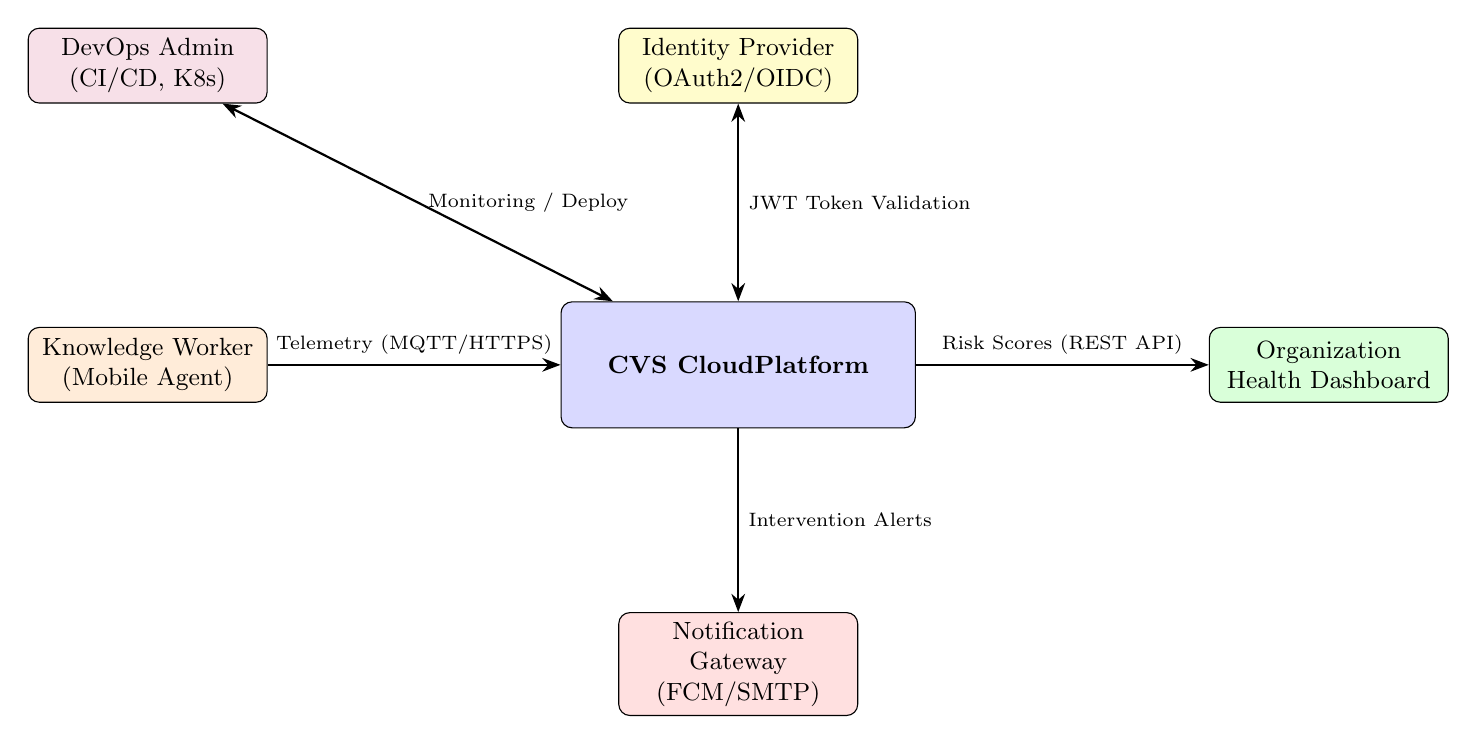
\begin{tikzpicture}

    %% Central system box
    \node[draw, rectangle, fill=blue!15, rounded corners,
          minimum width=4.5cm, minimum height=1.6cm, font=\bfseries\small,
          text centered]
          (sys) at (0,0) {CVS Cloud\\Platform};

    %% External actors — absolute positions
    \node[blockO, text width=2.8cm] (user)   at (-7.5,  0)   {Knowledge Worker\\(Mobile Agent)};
    \node[blockG, text width=2.8cm] (org)    at ( 7.5,  0)   {Organization\\Health Dashboard};
    \node[blockY, text width=2.8cm] (idp)    at ( 0,    3.8) {Identity Provider\\(OAuth2/OIDC)};
    \node[blockR, text width=2.8cm] (notif)  at ( 0,   -3.8) {Notification Gateway\\(FCM/SMTP)};
    \node[blockP, text width=2.8cm] (devops) at (-7.5,  3.8) {DevOps Admin\\(CI/CD, K8s)};

    %% Arrows
    \draw[arrow]  (user)   -- node[above, font=\scriptsize]{Telemetry (MQTT/HTTPS)}    (sys);
    \draw[arrow]  (sys)    -- node[above, font=\scriptsize]{Risk Scores (REST API)}     (org);
    \draw[darrow] (sys)    -- node[right, font=\scriptsize]{JWT Token Validation}       (idp);
    \draw[arrow]  (sys)    -- node[right, font=\scriptsize]{Intervention Alerts}        (notif);
    \draw[darrow] (devops) -- node[right, font=\scriptsize]{Monitoring / Deploy}       (sys);

  \end{tikzpicture}
  \caption{Level-0 Context Diagram: system boundary and external actor interactions.}
  \label{fig:context}
\end{figure}

\subsection{Four-Layer Component Architecture (Level 1)}

The platform's internal structure is organized into four horizontal processing layers,
each implementing a well-defined separation of concerns. This design follows the layered
architectural pattern, which reduces coupling between producers and consumers of telemetry
data and provides independent scalability for each processing stage \cite{b6}.
Figure~\ref{fig:layers} presents the Level-1 component diagram.

\begin{figure}[H]
  \centering
  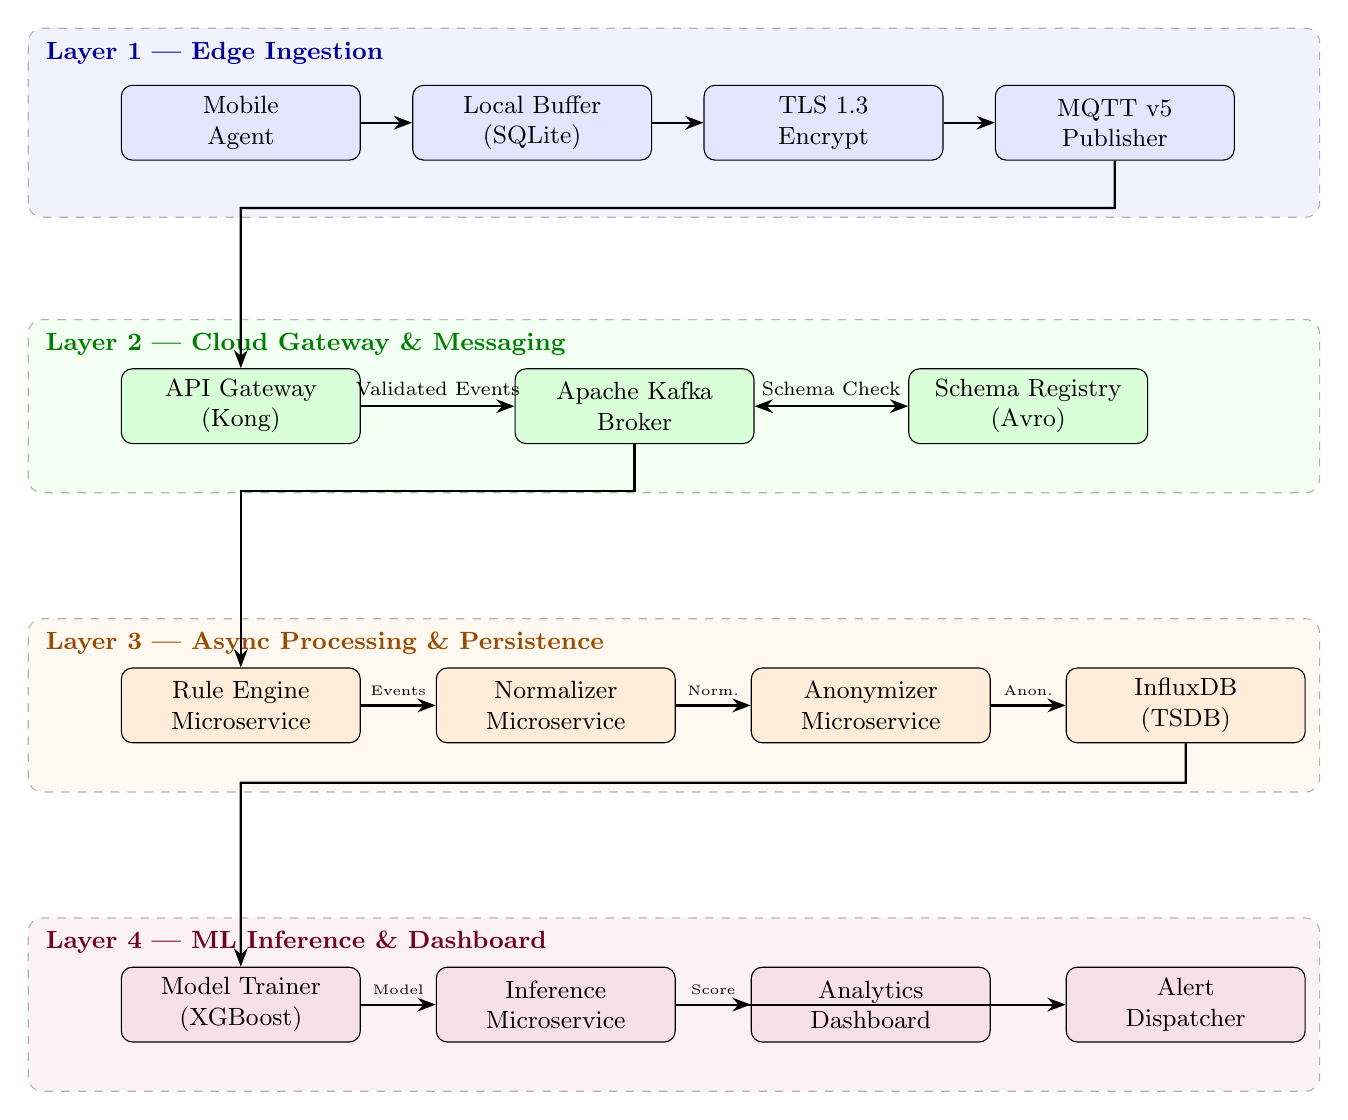
\begin{tikzpicture}[every node/.style={font=\small}]

    %% ===================== LAYER 1 =====================
    \draw[fill=blue!5, draw=gray!60, dashed, rounded corners=5pt]
         (-8.2, -1.2) rectangle (8.2, 1.2);
    \node[anchor=north west, font=\small\bfseries, text=blue!60!black]
         at (-8.1, 1.15) {Layer 1 \textemdash{} Edge Ingestion};

    \node[block, text width=2.8cm] (agent)  at (-5.5,  0) {Mobile\\Agent};
    \node[block, text width=2.8cm] (buf)    at (-1.8,  0) {Local Buffer\\(SQLite)};
    \node[block, text width=2.8cm] (tls)    at ( 1.9,  0) {TLS 1.3\\Encrypt};
    \node[block, text width=2.8cm] (mqtt)   at ( 5.6,  0) {MQTT v5\\Publisher};

    \draw[arrow] (agent) -- (buf);
    \draw[arrow] (buf)   -- (tls);
    \draw[arrow] (tls)   -- (mqtt);

    %% ===================== LAYER 2 =====================
    \draw[fill=green!5, draw=gray!60, dashed, rounded corners=5pt]
         (-8.2, -4.7) rectangle (8.2, -2.5);
    \node[anchor=north west, font=\small\bfseries, text=green!50!black]
         at (-8.1, -2.55) {Layer 2 \textemdash{} Cloud Gateway \& Messaging};

    \node[blockG, text width=2.8cm] (apigw)  at (-5.5, -3.6) {API Gateway\\(Kong)};
    \node[blockG, text width=2.8cm] (kafka)  at (-0.5, -3.6) {Apache Kafka\\Broker};
    \node[blockG, text width=2.8cm] (schema) at ( 4.5, -3.6) {Schema Registry\\(Avro)};

    %% Inter-layer arrow L1→L2
    \draw[arrow] (mqtt.south) -- ++(0,-0.6) -- ++(-11.1, 0) -- (apigw.north);

    \draw[arrow]  (apigw)  -- node[above, font=\scriptsize]{Validated Events} (kafka);
    \draw[darrow] (kafka)  -- node[above, font=\scriptsize]{Schema Check}     (schema);

    %% ===================== LAYER 3 =====================
    \draw[fill=orange!5, draw=gray!60, dashed, rounded corners=5pt]
         (-8.2, -8.5) rectangle (8.2, -6.3);
    \node[anchor=north west, font=\small\bfseries, text=orange!60!black]
         at (-8.1, -6.35) {Layer 3 \textemdash{} Async Processing \& Persistence};

    \node[blockO, text width=2.8cm] (rule)   at (-5.5, -7.4) {Rule Engine\\Microservice};
    \node[blockO, text width=2.8cm] (norm)   at (-1.5, -7.4) {Normalizer\\Microservice};
    \node[blockO, text width=2.8cm] (anon)   at ( 2.5, -7.4) {Anonymizer\\Microservice};
    \node[blockO, text width=2.8cm] (influx) at ( 6.5, -7.4) {InfluxDB\\(TSDB)};

    %% Inter-layer arrow L2→L3
    \draw[arrow] (kafka.south) -- ++(0,-0.6) -- ++(-5.0, 0) -- (rule.north);

    \draw[arrow] (rule)   -- node[above, font=\scriptsize]{\tiny Events} (norm);
    \draw[arrow] (norm)   -- node[above, font=\scriptsize]{\tiny Norm.}  (anon);
    \draw[arrow] (anon)   -- node[above, font=\scriptsize]{\tiny Anon.}  (influx);

    %% ===================== LAYER 4 =====================
    \draw[fill=purple!5, draw=gray!60, dashed, rounded corners=5pt]
         (-8.2, -12.3) rectangle (8.2, -10.1);
    \node[anchor=north west, font=\small\bfseries, text=purple!60!black]
         at (-8.1, -10.15) {Layer 4 \textemdash{} ML Inference \& Dashboard};

    \node[blockP, text width=2.8cm] (trainer) at (-5.5, -11.2) {Model Trainer\\(XGBoost)};
    \node[blockP, text width=2.8cm] (infer)   at (-1.5, -11.2) {Inference\\Microservice};
    \node[blockP, text width=2.8cm] (dash)    at ( 2.5, -11.2) {Analytics\\Dashboard};
    \node[blockP, text width=2.8cm] (alertD)  at ( 6.5, -11.2) {Alert\\Dispatcher};

    %% Inter-layer arrow L3→L4
    \draw[arrow] (influx.south) -- ++(0,-0.5) -- ++(-12.0, 0) -- (trainer.north);

    \draw[arrow] (trainer) -- node[above, font=\scriptsize]{\tiny Model}  (infer);
    \draw[arrow] (infer)   -- node[above, font=\scriptsize]{\tiny Score}  (dash);
    \draw[arrow] (infer.east) -- ++(0.2, 0) |- (alertD.west);

  \end{tikzpicture}
  \caption{Level-1 Four-Layer Component Diagram of the CVS Cloud Platform.}
  \label{fig:layers}
\end{figure}

\subsection{Layer Responsibilities}

\subsubsection{Layer 1 — Edge Ingestion}

The mobile agent is implemented as a battery-efficient background service. It polls
native device APIs at a configurable sampling frequency (default: one reading every
30~seconds) for three primary signals: (i)~ambient light level in lux from the device's
Ambient Light Sensor (ALS); (ii)~screen-to-device proximity distance in centimeters
from the proximity/ToF sensor; and (iii)~active screen interaction time derived from the
OS's \texttt{UsageStatsManager} (Android) or \texttt{CMMotionActivity} (iOS) APIs.
Readings are buffered locally in a SQLite micro-database and transmitted in micro-batches
every 5~minutes over TLS~1.3-encrypted MQTT~v5 channels. This micro-batch aggregation
strategy preserves battery life while maintaining the temporal granularity required
for the ML feature engineering pipeline \cite{b8}.

\subsubsection{Layer 2 — Cloud Gateway and Messaging}

Inbound telemetry micro-batches arrive at a Kong API Gateway instance responsible for
JWT authentication validation, rate limiting (maximum 100~requests/min per device),
and request routing \cite{b9}. Authenticated payloads are forwarded to a 3-replica
Apache Kafka broker cluster organized into partitioned topics. Kafka's distributed
commit log provides sub-millisecond latency at millions-of-events-per-second throughput,
while fully decoupling producer and consumer lifecycles \cite{b10}. A Confluent Schema
Registry enforces Avro message schemas, preventing schema drift from breaking downstream
consumers.

\subsubsection{Layer 3 — Asynchronous Processing and Persistence}

Three stateless microservices consume Kafka topics in parallel consumer groups:
(i)~the Rule Engine Microservice applies immediate 20-20-20 clinical threshold
evaluations; (ii)~the Normalizer Microservice applies z-score standardization per
sensor modality with linear forward-fill for missing readings; and (iii)~the Anonymizer
Microservice replaces device identifiers with pseudonymous UUIDs and injects
Laplace-distributed differential privacy noise ($\varepsilon = 1.0$) to all continuous
sensor fields \cite{b11}. Processed records are persisted to InfluxDB organized into
buckets, measurements, tags, and fields.

\subsubsection{Layer 4 — Machine Learning Inference}

A scheduled model trainer executes nightly as a Kubernetes CronJob, retrieving the
previous 30~days of anonymized records from InfluxDB, engineering a 9-feature matrix,
and training a Gradient Boosted Trees classifier (XGBoost~2.0) to produce a CVS Risk
Score $\in [0,1]$ for each user demographic profile. The serialized model artifact is
versioned in an S3-compatible object store. The stateless Inference Microservice
computes real-time scores as new telemetry arrives. The Alert Dispatcher triggers
Firebase Cloud Messaging (FCM) push notifications when a user's rolling 60-minute risk
score exceeds 0.70.

\subsection{Data-Flow Diagram}

Figure~\ref{fig:dataflow} presents the end-to-end data flow annotated with the
transformation applied at each stage.

\begin{figure}[H]
  \centering
  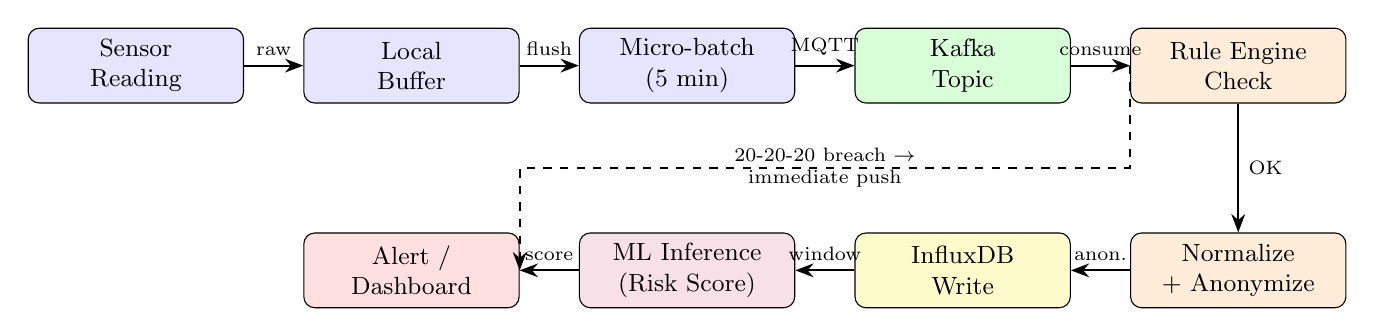
\begin{tikzpicture}[node distance=0cm, every node/.style={font=\small}]

    %% Row 1 (left to right)
    \node[block, text width=2.5cm]  (sensor) at ( 0,    0) {Sensor\\Reading};
    \node[block, text width=2.5cm]  (buf2)   at ( 3.5,  0) {Local\\Buffer};
    \node[block, text width=2.5cm]  (batch)  at ( 7.0,  0) {Micro-batch\\(5 min)};
    \node[blockG, text width=2.5cm] (kaf2)   at (10.5,  0) {Kafka\\Topic};
    \node[blockO, text width=2.5cm] (rule2)  at (14.0,  0) {Rule Engine\\Check};

    \draw[arrow] (sensor) -- node[above,font=\scriptsize]{raw} (buf2);
    \draw[arrow] (buf2)   -- node[above,font=\scriptsize]{flush} (batch);
    \draw[arrow] (batch)  -- node[above,font=\scriptsize]{MQTT} (kaf2);
    \draw[arrow] (kaf2)   -- node[above,font=\scriptsize]{consume} (rule2);

    %% Row 2 (right to left)
    \node[blockO, text width=2.5cm]  (norm2)  at (14.0, -2.6) {Normalize\\+ Anonymize};
    \node[blockY, text width=2.5cm]  (tsdb2)  at (10.5, -2.6) {InfluxDB\\Write};
    \node[blockP, text width=2.5cm]  (infer2) at ( 7.0, -2.6) {ML Inference\\(Risk Score)};
    \node[blockR, text width=2.5cm]  (alert2) at ( 3.5, -2.6) {Alert /\\Dashboard};

    \draw[arrow] (norm2)  -- node[above,font=\scriptsize]{anon.} (tsdb2);
    \draw[arrow] (tsdb2)  -- node[above,font=\scriptsize]{window} (infer2);
    \draw[arrow] (infer2) -- node[above,font=\scriptsize]{score} (alert2);

    %% Vertical connectors
    \draw[arrow] (rule2.south) -- node[right,font=\scriptsize]{OK} (norm2.north);

    %% Immediate alert: dashed line from rule2 bottom-left corner going left to alert2
    \draw[dasharrow] (rule2.west) -- ++(0, -1.3) -- (alert2.east |- 0,-1.3) -- (alert2.east);
    \node[font=\scriptsize, text width=4cm, align=center] at (8.75, -1.3)
         {20-20-20 breach $\rightarrow$ immediate push};

  \end{tikzpicture}
  \caption{End-to-End Data-Flow: from raw sensor reading to organizational intervention.}
  \label{fig:dataflow}
\end{figure}

\subsection{Deployment View — Cloud Infrastructure}

The platform is deployed on a managed Kubernetes cluster (AWS EKS or GCP GKE) organized
into three node pools: an \textit{ingestion pool} for API Gateway and Kafka Connect
workers, a \textit{processing pool} for stateless microservices, and a \textit{storage
pool} of SSD-backed persistent volumes for InfluxDB and the model artifact store.

\begin{figure}[H]
  \centering
  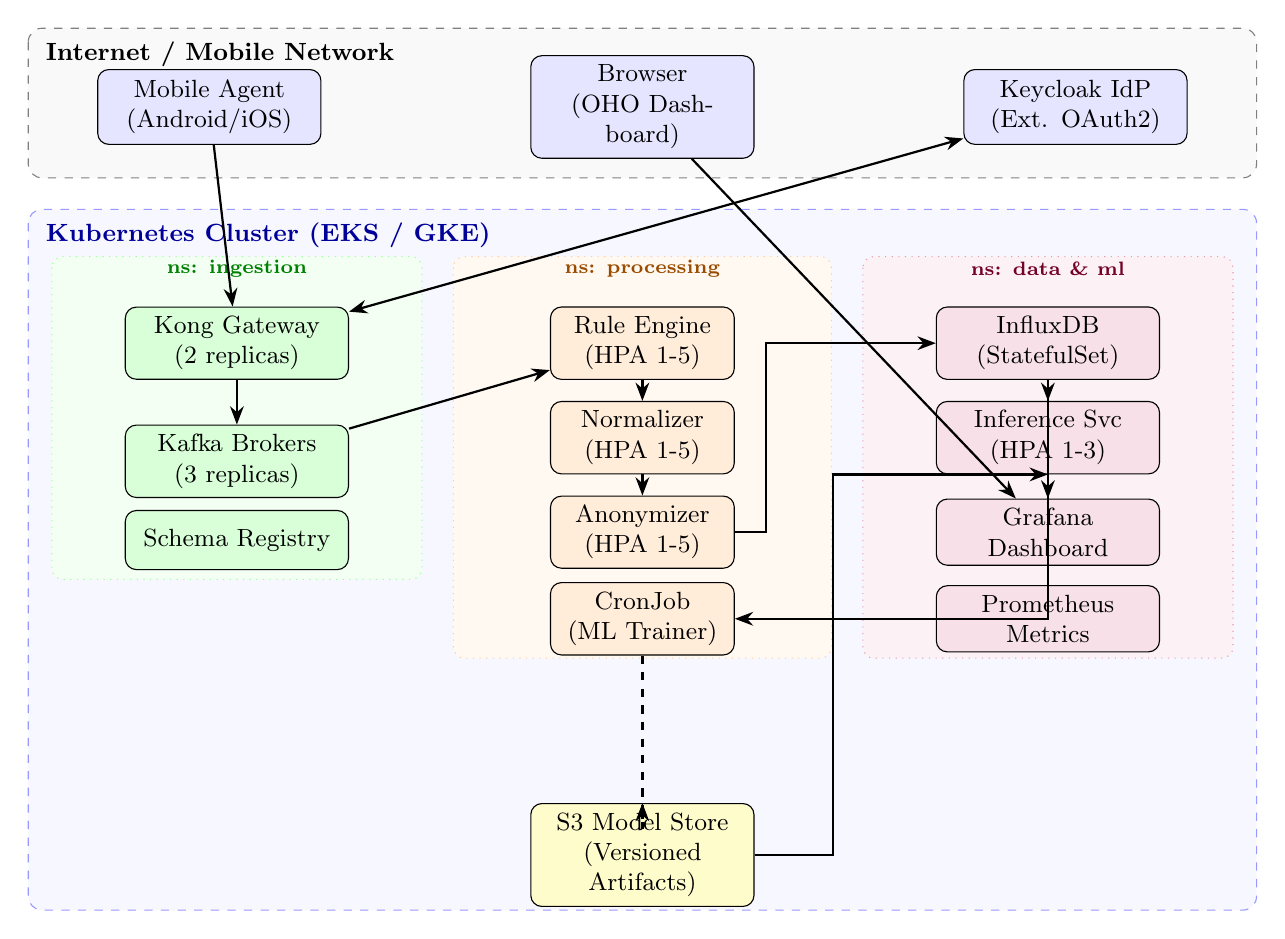
\begin{tikzpicture}[every node/.style={font=\small}]

    %% Internet boundary
    \draw[fill=gray!5, draw=gray, dashed, rounded corners=5pt]
         (-7.8, 2.0) rectangle (7.8, 0.1);
    \node[anchor=north west, font=\small\bfseries] at (-7.7, 1.95) {Internet / Mobile Network};

    \node[block, text width=2.6cm] (mob)  at (-5.5, 1.0) {Mobile Agent\\(Android/iOS)};
    \node[block, text width=2.6cm] (web)  at ( 0.0, 1.0) {Browser\\(OHO Dashboard)};
    \node[block, text width=2.6cm] (ext)  at ( 5.5, 1.0) {Keycloak IdP\\(Ext. OAuth2)};

    %% K8s cluster boundary
    \draw[fill=blue!3, draw=blue!40, dashed, rounded corners=5pt]
         (-7.8, -0.3) rectangle (7.8, -9.2);
    \node[anchor=north west, font=\small\bfseries, text=blue!60!black]
         at (-7.7, -0.35) {Kubernetes Cluster (EKS / GKE)};

    %% NS: ingestion
    \draw[fill=green!5, draw=green!40, dotted, rounded corners=4pt]
         (-7.5, -0.9) rectangle (-2.8, -5.0);
    \node[font=\scriptsize\bfseries, text=green!50!black] at (-5.15, -1.05) {ns: ingestion};
    \node[blockG, text width=2.6cm, minimum height=0.75cm] (kong2)  at (-5.15, -2.0) {Kong Gateway\\(2 replicas)};
    \node[blockG, text width=2.6cm, minimum height=0.75cm] (kafka3) at (-5.15, -3.5) {Kafka Brokers\\(3 replicas)};
    \node[blockG, text width=2.6cm, minimum height=0.75cm] (sr2)    at (-5.15, -4.5) {Schema Registry};

    %% NS: processing
    \draw[fill=orange!5, draw=orange!40, dotted, rounded corners=4pt]
         (-2.4, -0.9) rectangle (2.4, -6.0);
    \node[font=\scriptsize\bfseries, text=orange!60!black] at (0.0, -1.05) {ns: processing};
    \node[blockO, text width=2.1cm, minimum height=0.7cm] (ruleP) at (0.0, -2.0) {Rule Engine\\(HPA 1-5)};
    \node[blockO, text width=2.1cm, minimum height=0.7cm] (normP) at (0.0, -3.2) {Normalizer\\(HPA 1-5)};
    \node[blockO, text width=2.1cm, minimum height=0.7cm] (anonP) at (0.0, -4.4) {Anonymizer\\(HPA 1-5)};
    \node[blockO, text width=2.1cm, minimum height=0.7cm] (cronP) at (0.0, -5.5) {CronJob\\(ML Trainer)};

    %% NS: data \& ml
    \draw[fill=purple!5, draw=purple!40, dotted, rounded corners=4pt]
         (2.8, -0.9) rectangle (7.5, -6.0);
    \node[font=\scriptsize\bfseries, text=purple!60!black] at (5.15, -1.05) {ns: data \& ml};
    \node[blockP, text width=2.6cm, minimum height=0.7cm] (influx2) at (5.15, -2.0) {InfluxDB\\(StatefulSet)};
    \node[blockP, text width=2.6cm, minimum height=0.7cm] (inferP2) at (5.15, -3.2) {Inference Svc\\(HPA 1-3)};
    \node[blockP, text width=2.6cm, minimum height=0.7cm] (grafana) at (5.15, -4.4) {Grafana\\Dashboard};
    \node[blockP, text width=2.6cm, minimum height=0.7cm] (prom)    at (5.15, -5.5) {Prometheus\\Metrics};

    %% S3 external (below cluster)
    \node[blockY, text width=2.6cm] (s3) at (0.0, -8.5) {S3 Model Store\\(Versioned Artifacts)};
    \draw[dasharrow] (cronP.south) -- ++(0,-0.7) -- ++(0,-1.5) -- (s3.north);
    \draw[arrow]     (s3.east)     -- ++(1.0, 0) |- (inferP2.south);

    %% Connections
    \draw[arrow]  (mob)    -- (kong2);
    \draw[arrow]  (web)    -- (grafana);
    \draw[darrow] (ext)    -- (kong2);
    \draw[arrow]  (kong2)  -- (kafka3);
    \draw[arrow]  (kafka3) -- (ruleP);
    \draw[arrow]  (ruleP)  -- (normP);
    \draw[arrow]  (normP)  -- (anonP);
    \draw[arrow]  (anonP.east)  -- ++(0.4, 0) |- (influx2.west);
    \draw[arrow]  (influx2) -- (inferP2);
    \draw[arrow]  (inferP2) -- (grafana);
    \draw[arrow]  (influx2.south) -- ++(0,-0.4) |- (cronP.east);

  \end{tikzpicture}
  \caption{Deployment View: Kubernetes namespaces, node pools, and external dependencies.}
  \label{fig:deploy}
\end{figure}

\subsection{Security Architecture View}

Security is treated as a cross-cutting concern enforced at four independent layers.
Figure~\ref{fig:security} illustrates the layered security enforcement model.

\begin{figure}[H]
  \centering
  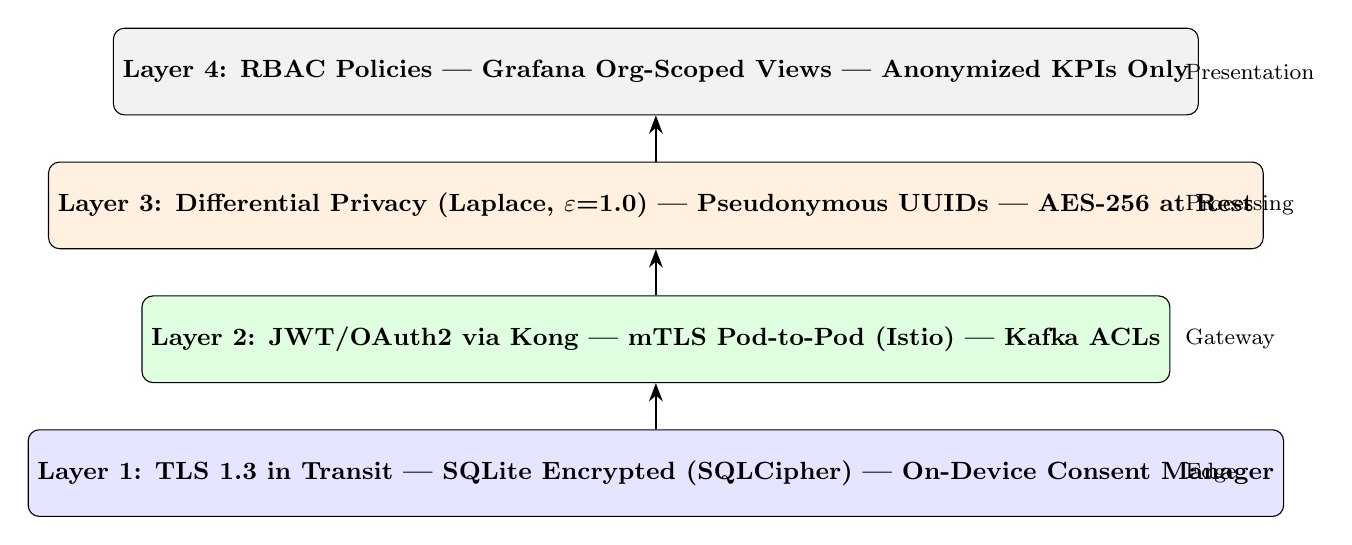
\begin{tikzpicture}[every node/.style={font=\small}]

    \node[draw, fill=gray!10,   rounded corners, minimum width=13cm, minimum height=1.1cm,
          text centered, font=\small\bfseries] (l4s) at (0, 0)
      {Layer 4: RBAC Policies | Grafana Org-Scoped Views | Anonymized KPIs Only};

    \node[draw, fill=orange!12, rounded corners, minimum width=13cm, minimum height=1.1cm,
          text centered, font=\small\bfseries] (l3s) at (0, -1.7)
      {Layer 3: Differential Privacy (Laplace, $\varepsilon$=1.0) | Pseudonymous UUIDs | AES-256 at Rest};

    \node[draw, fill=green!12,  rounded corners, minimum width=13cm, minimum height=1.1cm,
          text centered, font=\small\bfseries] (l2s) at (0, -3.4)
      {Layer 2: JWT/OAuth2 via Kong | mTLS Pod-to-Pod (Istio) | Kafka ACLs};

    \node[draw, fill=blue!10,   rounded corners, minimum width=13cm, minimum height=1.1cm,
          text centered, font=\small\bfseries] (l1s) at (0, -5.1)
      {Layer 1: TLS 1.3 in Transit | SQLite Encrypted (SQLCipher) | On-Device Consent Manager};

    \draw[arrow] (l1s) -- (l2s);
    \draw[arrow] (l2s) -- (l3s);
    \draw[arrow] (l3s) -- (l4s);

    \node[font=\footnotesize, anchor=west] at ( 6.6,  0)    {Presentation};
    \node[font=\footnotesize, anchor=west] at ( 6.6, -1.7)  {Processing};
    \node[font=\footnotesize, anchor=west] at ( 6.6, -3.4)  {Gateway};
    \node[font=\footnotesize, anchor=west] at ( 6.6, -5.1)  {Edge};

  \end{tikzpicture}
  \caption{Layered Security Architecture: enforcement points across all four platform layers.}
  \label{fig:security}
\end{figure}

The security design is grounded in three regulatory principles. First, GDPR Article~5
mandates data minimization and purpose limitation \cite{b12}: the platform collects only
the three non-invasive sensor signals strictly necessary for CVS risk estimation.
Second, privacy-by-design is enforced at the Anonymizer Microservice through Laplace-
distributed noise with $\varepsilon = 1.0$, consistent with the GDPR-compliance
framework established for healthcare AI by Alotaibi et al.\ \cite{b11}. Third, Federated
Learning is designated as the long-term evolution of the model pipeline, keeping raw data
entirely within institutional boundaries \cite{b13,b14}.

%% ============================================================
\section{Prototype Architecture}
%% ============================================================

\subsection{Technology Stack Summary}

Table~\ref{tab:stack} consolidates the technology selections for each component with the
primary technical justification for each choice.

\begin{table}[H]
  \centering
  \caption{Prototype Technology Stack}
  \label{tab:stack}
  \begin{tabularx}{\textwidth}{>{\bfseries}p{3.5cm} p{3.5cm} X}
    \toprule
    \textbf{Component} & \textbf{Technology} & \textbf{Primary Justification} \\
    \midrule
    Mobile Agent & Kotlin + WorkManager & Battery-efficient background scheduling;
      guaranteed micro-batch execution without foreground service \\
    Transport Protocol & MQTT v5 (Mosquitto) & Lightweight IoT publish-subscribe;
      QoS-1 guaranteed delivery; minimal overhead per message \cite{b8} \\
    API Gateway & Kong Gateway 3.x & Plugin-based JWT validation, rate limiting, request
      transformation; native Kubernetes Ingress support \cite{b9} \\
    Message Broker & Apache Kafka 3.6 & Sub-ms latency; billions events/day;
      exactly-once semantics; decoupled producers/consumers \cite{b10} \\
    Schema Enforcement & Confluent Schema Registry (Avro) & Backward-compatible
      schema evolution; binary serialization $\approx$40\% smaller than JSON \\
    Processing Microservices & Python 3.11 + FastAPI & ASGI async handling;
      native scikit-learn/pandas integration; rapid iteration \\
    Time-Series Database & InfluxDB 2.7 OSS & Write-heavy IoT workload performance;
      native retention policies; Flux query language; Grafana plugin \cite{b7} \\
    ML Framework & scikit-learn 1.4 + XGBoost 2.0 & GBT outperforms neural nets on
      tabular small-feature datasets \cite{b19}; sub-100~ms inference without GPU \\
    Container Orchestration & Kubernetes 1.29 (EKS) & HPA elastic scaling; RBAC
      namespace isolation; rolling deployments \cite{b20} \\
    Service Mesh & Istio 1.20 & mTLS for all pod traffic; traffic policy; Zipkin tracing \\
    Observability & Prometheus + Grafana & Time-series metrics; pre-built Kafka and
      Kubernetes dashboards; alert manager integration \\
    CI/CD & GitHub Actions + Helm 3 & Automated build, test, push, and rolling deploy \\
    \bottomrule
  \end{tabularx}
\end{table}

\subsection{Edge Agent Sensor Sampling and Data Schema}

Table~\ref{tab:sensors} specifies the three sensor modalities collected by the mobile
agent and their clinical justification.

\begin{table}[H]
  \centering
  \caption{Edge Sensor Sampling Plan}
  \label{tab:sensors}
  \begin{tabularx}{\textwidth}{p{3.2cm} p{3.8cm} p{2cm} p{1.8cm} X}
    \toprule
    \textbf{Signal} & \textbf{Native API} & \textbf{Unit} & \textbf{Interval} &
    \textbf{Clinical Relevance} \\
    \midrule
    Ambient Light & ALS (\texttt{Sensor.TYPE\_LIGHT}) & lux & 30 s &
      Lux mismatch is a primary ergonomic trigger \cite{b3} \\
    Screen-to-Eye Distance & Proximity / ToF sensor & cm & 30 s &
      Distance $<$30~cm exponentially increases accommodation strain \cite{b3} \\
    Active Screen Time & \texttt{UsageStatsManager} & min & 5 min &
      Session duration is the strongest CVS onset predictor \cite{b18} \\
    \bottomrule
  \end{tabularx}
\end{table}

The Avro schema for a telemetry micro-batch is defined below:

\begin{lstlisting}[language=json, caption={Avro Schema — TelemetryBatch},
  basicstyle=\ttfamily\footnotesize, frame=single, numbers=left]
{
  "type": "record",
  "name": "TelemetryBatch",
  "namespace": "edu.escuelaing.cvs",
  "fields": [
    { "name": "device_uuid",     "type": "string" },
    { "name": "batch_timestamp", "type": "long",
      "logicalType": "timestamp-millis" },
    { "name": "readings", "type": {
        "type": "array",
        "items": {
          "type": "record",
          "name": "SensorReading",
          "fields": [
            { "name": "sensor_type", "type": {
                "type": "enum", "name": "SensorType",
                "symbols": ["AMBIENT_LIGHT","PROXIMITY","SCREEN_TIME"]
            }},
            { "name": "value",      "type": "float"  },
            { "name": "unit",       "type": "string" },
            { "name": "sampled_at", "type": "long",
              "logicalType": "timestamp-millis" }
          ]
        }
    }},
    { "name": "app_version",  "type": "string" },
    { "name": "consent_hash", "type": "string",
      "doc": "SHA-256 of user-signed consent document" }
  ]
}
\end{lstlisting}

\subsection{Kafka Topic Design}

\begin{table}[H]
  \centering
  \caption{Kafka Topic Design}
  \label{tab:topics}
  \begin{tabularx}{\textwidth}{p{5cm} p{1.8cm} p{1.8cm} X}
    \toprule
    \textbf{Topic Name} & \textbf{Partitions} & \textbf{Replicas} & \textbf{Purpose} \\
    \midrule
    \texttt{cvs.telemetry.raw}        & 12 & 3 &
      Receives validated Avro micro-batches from API Gateway \\
    \texttt{cvs.telemetry.normalized} & 12 & 3 &
      Z-scored, anonymized records from Normalizer+Anonymizer microservices \\
    \texttt{cvs.alerts.immediate}     &  6 & 3 &
      20-20-20 rule violations requiring real-time push notification \\
    \texttt{cvs.inference.scores}     &  6 & 3 &
      CVS Risk Scores produced by the Inference Microservice \\
    \bottomrule
  \end{tabularx}
\end{table}

Partition count of 12 for the ingestion topics is calibrated to support the expected
maximum of 10,000 concurrent device connections per organizational tenant. With Kafka's
documented throughput of millions of events per second across a 3-broker cluster
\cite{b10}, 12 partitions provide a safety margin of approximately 10x the expected
peak load.

\subsection{InfluxDB Data Model}

\begin{table}[H]
  \centering
  \caption{InfluxDB Measurement Schema: \texttt{sensor\_readings}}
  \label{tab:influx}
  \begin{tabularx}{\textwidth}{p{2.5cm} p{3.5cm} p{2cm} X}
    \toprule
    \textbf{Element} & \textbf{Name} & \textbf{Type} & \textbf{Description} \\
    \midrule
    Tag & \texttt{device\_uuid}  & String & Pseudonymous device identifier \\
    Tag & \texttt{org\_unit}     & String & Hashed organizational unit code \\
    Tag & \texttt{sensor\_type}  & String & AMBIENT\_LIGHT, PROXIMITY, SCREEN\_TIME \\
    Tag & \texttt{device\_class} & String & phone, tablet, laptop \\
    \midrule
    Field & \texttt{raw\_value}        & Float   & Original sensor reading \\
    Field & \texttt{normalized\_value} & Float   & Z-scored: $(\mu=0,\,\sigma=1)$ \\
    Field & \texttt{noised\_value}     & Float   & DP-perturbed ($\varepsilon=1.0$) \\
    Field & \texttt{quality\_flag}     & Integer & 0=OK, 1=interpolated, 2=out-of-range \\
    \midrule
    Timestamp & \texttt{\_time} & ns (UTC) & Kafka ingestion timestamp \\
    \bottomrule
  \end{tabularx}
\end{table}

InfluxDB 2.7 was selected over TimescaleDB because the platform's workload is
write-dominant with time-range aggregation queries, where InfluxDB's line protocol and
compaction strategy provide documented throughput advantages \cite{b7}. TimescaleDB
would be preferred if complex relational joins with user metadata were a primary access
pattern---a scenario not present in the current prototype scope.

\subsection{Machine Learning Pipeline}

\subsubsection{Feature Engineering}

The model trainer constructs a 30-day feature window per pseudonymous UUID:

\begin{lstlisting}[language=bash, caption={Flux Query for 30-Day Feature Window},
  basicstyle=\ttfamily\footnotesize, frame=single, numbers=left]
from(bucket: "cvs_platform")
  |> range(start: -30d)
  |> filter(fn: (r) => r["_measurement"] == "sensor_readings")
  |> filter(fn: (r) => r["device_uuid"] == param_uuid)
  |> aggregateWindow(every: 1h, fn: mean, createEmpty: false)
  |> pivot(rowKey: ["_time"],
           columnKey: ["sensor_type"],
           valueColumn: "_value")
\end{lstlisting}

The resulting feature matrix $\mathbf{X} \in \mathbb{R}^{n \times 9}$ contains the
features described in Table~\ref{tab:features}.

\begin{table}[H]
  \centering
  \caption{CVS Risk Score Model: Feature Matrix}
  \label{tab:features}
  \begin{tabularx}{\textwidth}{p{0.6cm} p{4.5cm} X}
    \toprule
    \textbf{\#} & \textbf{Feature} & \textbf{Description} \\
    \midrule
    1 & \texttt{mean\_lux\_daily}        & Mean daily ambient lux level \\
    2 & \texttt{std\_lux\_daily}         & Lux standard deviation (lighting variability) \\
    3 & \texttt{mean\_proximity\_cm}     & Mean screen-to-eye distance in active sessions \\
    4 & \texttt{min\_proximity\_cm}      & Minimum proximity (worst-case posture) \\
    5 & \texttt{total\_screen\_min}      & Total daily screen time in minutes \\
    6 & \texttt{max\_cont\_session\_min} & Longest continuous session without 20~min break \\
    7 & \texttt{lux\_screen\_ratio}      & Ambient lux to estimated screen brightness ratio \\
    8 & \texttt{evening\_screen\_ratio}  & Fraction of screen time occurring after 20:00 \\
    9 & \texttt{break\_compliance\_score}& Fraction of 20-min intervals with $\geq$3~min break \\
    \bottomrule
  \end{tabularx}
\end{table}

\subsubsection{Model Selection and Training}

XGBoost Gradient Boosted Trees are adopted over neural network alternatives for three
reasons: (i)~tabular sensor data with a small number of engineered features consistently
favors tree-based ensembles in low-resource settings \cite{b19}; (ii)~gradient-boosted
models produce interpretable feature importance scores suitable for clinical validation;
(iii)~inference latency is in the millisecond range without GPU hardware, compatible
with the sub-100~ms SLO defined in Section~XII.

Training follows a stratified 5-fold cross-validation strategy. The CVS Risk Score
label $y \in \{0,1\}$ is constructed synthetically: a user is labeled high-risk
($y=1$) if \texttt{break\_compliance\_score} $< 0.40$ AND
\texttt{max\_cont\_session\_min} $> 45$ simultaneously, consistent with the
physiological thresholds from Sheppard and Wolffsohn \cite{b2}.

Figure~\ref{fig:mlpipeline} presents the complete ML pipeline diagram.

\begin{figure}[H]
  \centering
  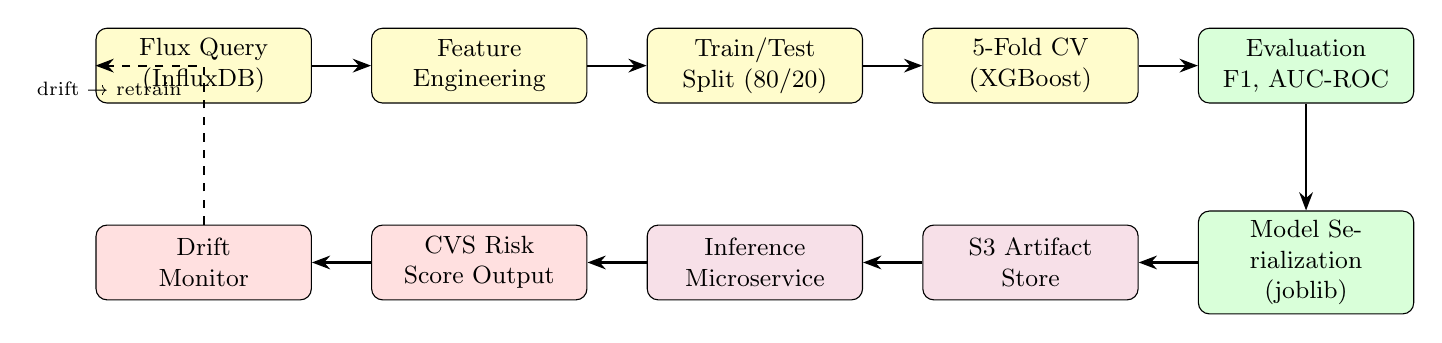
\begin{tikzpicture}[every node/.style={font=\small}]

    %% Top row: data→model
    \node[blockY, text width=2.5cm] (q)   at ( 0,    0) {Flux Query\\(InfluxDB)};
    \node[blockY, text width=2.5cm] (eng) at ( 3.5,  0) {Feature\\Engineering};
    \node[blockY, text width=2.5cm] (spl) at ( 7.0,  0) {Train/Test\\Split (80/20)};
    \node[blockY, text width=2.5cm] (cv)  at (10.5,  0) {5-Fold CV\\(XGBoost)};
    \node[blockG, text width=2.5cm] (ev)  at (14.0,  0) {Evaluation\\F1, AUC-ROC};

    \draw[arrow] (q) -- (eng);
    \draw[arrow] (eng) -- (spl);
    \draw[arrow] (spl) -- (cv);
    \draw[arrow] (cv)  -- (ev);

    %% Bottom row: deploy→inference (right to left)
    \node[blockG, text width=2.5cm] (ser)  at (14.0, -2.5) {Model Serialization\\(joblib)};
    \node[blockP, text width=2.5cm] (s3b)  at (10.5, -2.5) {S3 Artifact\\Store};
    \node[blockP, text width=2.5cm] (inf)  at ( 7.0, -2.5) {Inference\\Microservice};
    \node[blockR, text width=2.5cm] (sc)   at ( 3.5, -2.5) {CVS Risk\\Score Output};
    \node[blockR, text width=2.5cm] (mon)  at ( 0,   -2.5) {Drift\\Monitor};

    \draw[arrow] (ser) -- (s3b);
    \draw[arrow] (s3b) -- (inf);
    \draw[arrow] (inf) -- (sc);
    \draw[arrow] (sc)  -- (mon);

    %% Vertical connectors
    \draw[arrow] (ev.south) -- (ser.north);

    %% Retrain loop
    \draw[dasharrow] (mon.north) -- ++(0, 1.0) -- ++(-0.0, 0) |- (q.west);
    \node[font=\scriptsize, anchor=south] at (-1.2, -0.5) {drift → retrain};

  \end{tikzpicture}
  \caption{Machine Learning Pipeline: from InfluxDB query to CVS Risk Score inference.}
  \label{fig:mlpipeline}
\end{figure}

\subsection{REST API Specification}

\begin{table}[H]
  \centering
  \caption{REST API Endpoint Specification (v1)}
  \label{tab:api}
  \begin{tabularx}{\textwidth}{p{1.3cm} p{5.5cm} p{2.2cm} X}
    \toprule
    \textbf{Method} & \textbf{Endpoint} & \textbf{Auth} & \textbf{Description} \\
    \midrule
    POST & \texttt{/v1/telemetry/ingest}            & JWT &
      Accepts Avro micro-batch; publishes to \texttt{cvs.telemetry.raw} \\
    GET  & \texttt{/v1/scores/\{uuid\}/current}     & JWT &
      Returns current CVS Risk Score and top-3 feature importances \\
    GET  & \texttt{/v1/org/\{org\_id\}/risk-summary} & JWT + RBAC &
      Returns organizational risk distribution (P25, P50, P75, P95) \\
    POST & \texttt{/v1/alerts/acknowledge}           & JWT &
      Marks alert acknowledged; suppresses duplicate notifications for 4 h \\
    GET  & \texttt{/v1/health}                       & None &
      Kubernetes liveness and readiness probe endpoint \\
    DELETE & \texttt{/v1/users/\{uuid\}}             & JWT + RBAC &
      GDPR right-to-erasure: triggers pseudonymous UUID deletion across all stores \\
    \bottomrule
  \end{tabularx}
\end{table}

\subsection{Kubernetes Deployment Manifests and Scaling Policy}

\begin{lstlisting}[language=yaml, caption={Helm Values: HPA and Persistence Configuration},
  basicstyle=\ttfamily\footnotesize, frame=single, numbers=left]
# values.yaml (excerpt)
normalizer:
  replicaCount: 2
  hpa:
    enabled: true
    minReplicas: 1
    maxReplicas: 8
    targetCPUUtilizationPercentage: 60

inferenceSvc:
  replicaCount: 1
  hpa:
    enabled: true
    minReplicas: 1
    maxReplicas: 4
    targetCPUUtilizationPercentage: 70

kafka:
  replicaCount: 3
  persistence:
    enabled: true
    storageClass: "gp3"
    size: "50Gi"

influxdb:
  persistence:
    enabled: true
    storageClass: "gp3"
    size: "100Gi"
  retentionDays: 90
\end{lstlisting}

\subsection{Sequence Diagram: Alert Generation Lifecycle}

Figure~\ref{fig:sequence} presents the sequence diagram for the complete alert
generation lifecycle from sensor reading to push notification delivery.

\begin{figure}[H]
  \centering
  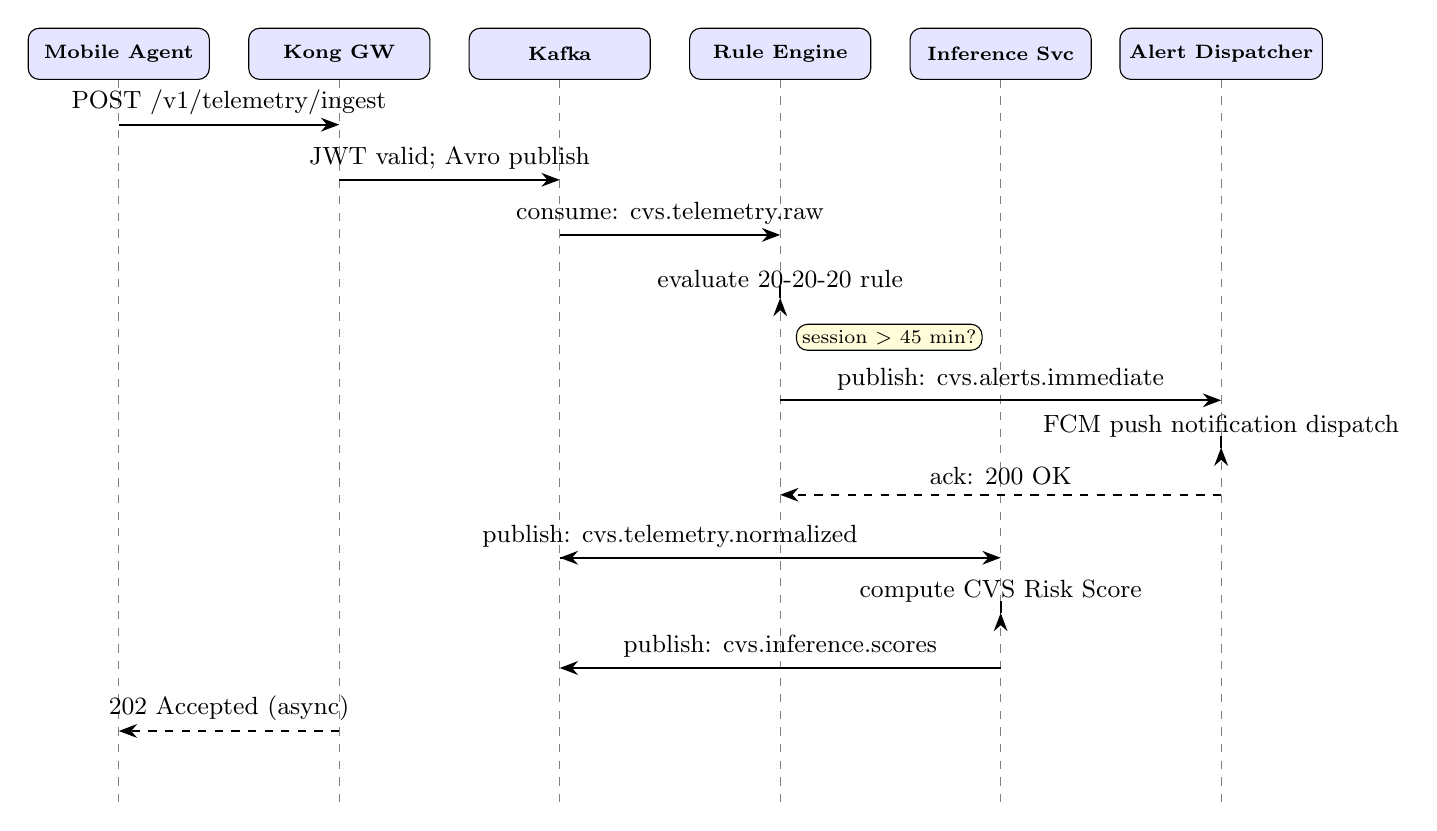
\begin{tikzpicture}[every node/.style={font=\scriptsize}]

    %% Lifeline headers
    \foreach \x/\lbl in {
      0/{Mobile Agent},
      2.8/{Kong GW},
      5.6/{Kafka},
      8.4/{Rule Engine},
      11.2/{Inference Svc},
      14.0/{Alert Dispatcher}}
    {
      \node[draw, fill=blue!10, rounded corners, minimum width=2.3cm, minimum height=0.65cm,
            font=\scriptsize\bfseries, text centered] at (\x, 0) {\lbl};
      \draw[dashed, gray] (\x, -0.33) -- (\x, -9.5);
    }

    %% Messages
    \draw[thick,->,>=Stealth] (0,-0.9)  -- node[above]{\small POST /v1/telemetry/ingest} (2.8,-0.9);
    \draw[thick,->,>=Stealth] (2.8,-1.6)-- node[above]{\small JWT valid; Avro publish}   (5.6,-1.6);
    \draw[thick,->,>=Stealth] (5.6,-2.3)-- node[above]{\small consume: cvs.telemetry.raw}(8.4,-2.3);

    \draw[thick,->,>=Stealth] (8.4,-3.1)-- node[above]{\small evaluate 20-20-20 rule}    (8.4,-3.1);
    \node[draw, fill=yellow!15, rounded corners, font=\scriptsize, inner sep=2pt,
          anchor=west] at (8.6,-3.6) {session $>$ 45 min?};

    %% Threshold breach path
    \draw[thick,->,>=Stealth] (8.4,-4.4) -- node[above]{\small publish: cvs.alerts.immediate} (14.0,-4.4);
    \draw[thick,->,>=Stealth] (14.0,-5.0)-- node[above]{\small FCM push notification dispatch} (14.0,-5.0);
    \draw[thick,dashed,->,>=Stealth] (14.0,-5.6)-- node[above]{\small ack: 200 OK} (8.4,-5.6);

    %% Normal processing path
    \draw[thick,->,>=Stealth] (8.4,-6.4) -- node[above]{\small publish: cvs.telemetry.normalized} (5.6,-6.4);
    \draw[thick,->,>=Stealth] (5.6,-6.4) -- node[above]{} (11.2,-6.4);
    \draw[thick,->,>=Stealth] (11.2,-7.1)-- node[above]{\small compute CVS Risk Score}          (11.2,-7.1);
    \draw[thick,->,>=Stealth] (11.2,-7.8)-- node[above]{\small publish: cvs.inference.scores}   (5.6,-7.8);

    %% Return to client
    \draw[thick,dashed,->,>=Stealth] (2.8,-8.6)-- node[above]{\small 202 Accepted (async)} (0,-8.6);

  \end{tikzpicture}
  \caption{Sequence Diagram: telemetry ingestion and alert generation lifecycle.}
  \label{fig:sequence}
\end{figure}

%% ============================================================
\section{Applied Microservices Design Patterns}
%% ============================================================

The CVS platform deliberately applies four established microservices design patterns
to address the distributed systems challenges inherent in high-throughput IoT telemetry
processing \cite{b28,b29}. This section documents each pattern, its motivation, and
its concrete realization in the prototype.

\subsection{Database-per-Service Pattern}

\textbf{Motivation.} In a microservices architecture, sharing a single database across
multiple services introduces tight coupling: a schema change in one service can break
another, and a database overload caused by one service degrades all others \cite{b29}.

\textbf{Realization.} Each microservice in Layer~3 operates on its own data boundary.
The Rule Engine operates exclusively on in-memory Kafka message state without
persisting to any database. The Normalizer and Anonymizer Microservices each maintain
stateless transformation logic and write their outputs exclusively to the next Kafka
topic in the pipeline---they never directly query InfluxDB. Only the persistence
microservice (InfluxDB writer) has write access to the time-series store. The Inference
Microservice has read-only access to InfluxDB and read-only access to the S3 model
artifact store. This strict access boundary prevents cross-service data coupling
and allows each service to be deployed, scaled, and replaced independently.

\subsection{Event Sourcing with Kafka as Immutable Log}

\textbf{Motivation.} Traditional CRUD-based architectures store only the current state
of an entity, making it difficult to reconstruct historical state, debug processing
errors, or replay events after a consumer failure \cite{b28}.

\textbf{Realization.} Apache Kafka's partitioned commit log serves as the event source
for the entire telemetry processing pipeline. All state changes---from raw sensor
reading to normalized record to inference score---are captured as a sequence of immutable
events in the Kafka topics. The configurable log retention period (default: 7~days for
\texttt{cvs.telemetry.raw}) allows any consumer to replay missed events from any
point in the recent past without requiring re-ingestion from mobile agents. This property
is critical for the ML training pipeline: if a model trainer job fails mid-execution,
it can resume from the last committed Kafka offset rather than losing all consumed
records. InfluxDB then acts as the materialized view of the Kafka event stream,
providing efficient time-range query access to the processed sensor history.

\subsection{CQRS (Command Query Responsibility Segregation)}

\textbf{Motivation.} The telemetry ingestion path (writes) and the analytics dashboard
path (reads) have fundamentally different performance characteristics: writes are
high-throughput, low-latency, and structurally simple (raw sensor records), while reads
are complex aggregations over time ranges across millions of records \cite{b28}.
Forcing both through the same data layer would create performance contention and
architectural coupling.

\textbf{Realization.} The platform implements CQRS at the Kafka topic level. The write
model is the \texttt{cvs.telemetry.raw} topic, optimized for high-throughput sequential
append. The read model is InfluxDB, which receives only processed, anonymized records
via the \texttt{cvs.telemetry.normalized} topic and is optimized for time-range
aggregation queries. The REST API enforces this separation explicitly: the
\texttt{POST /v1/telemetry/ingest} endpoint (command path) routes exclusively to Kafka,
while the \texttt{GET /v1/scores/\{uuid\}/current} and
\texttt{GET /v1/org/\{org\_id\}/risk-summary} endpoints (query path) route exclusively
to InfluxDB and the Inference Microservice. The read and write paths never share a
processing component, enabling independent horizontal scaling of each path.

\subsection{Circuit Breaker Pattern (via Istio)}

\textbf{Motivation.} In a distributed system with many inter-service calls, a single
failing service can cascade failures to all dependent services through repeated
connection attempts and timeout accumulation---a problem known as cascading failure
\cite{b29}. The Circuit Breaker pattern prevents this by monitoring failure rates and
temporarily blocking calls to a failing service, allowing it to recover.

\textbf{Realization.} The Istio service mesh enforces Circuit Breaker behavior through
its \texttt{DestinationRule} custom resources. Table~\ref{tab:circuitbreaker} specifies
the circuit breaker configuration for the three critical inter-service communication
pairs.

\begin{table}[H]
  \centering
  \caption{Circuit Breaker Configuration via Istio DestinationRule}
  \label{tab:circuitbreaker}
  \begin{tabularx}{\textwidth}{p{4cm} p{2.5cm} p{2.5cm} X}
    \toprule
    \textbf{Service Pair} & \textbf{Consecutive Errors} & \textbf{Ejection Time} &
    \textbf{Behavior on Open} \\
    \midrule
    Kong GW $\rightarrow$ Kafka & 5 & 30 s & Return 503 to mobile agent; agent retries after TTL \\
    Normalizer $\rightarrow$ InfluxDB & 3 & 60 s & Pause normalization; buffer events in Kafka \\
    Inference Svc $\rightarrow$ S3 & 3 & 120 s & Serve stale model from memory cache \\
    \bottomrule
  \end{tabularx}
\end{table}

The stale model cache for the Inference Microservice is a particularly important
resilience mechanism: if the S3 store becomes unavailable during a model artifact
refresh, the inference service continues serving the last successfully loaded model
version without interruption, maintaining the \texttt{cvs.inference.scores} output
topic with a small accuracy penalty acknowledged in the risk score metadata field.

%% ============================================================
\section{CI/CD Pipeline and DevOps Architecture}
%% ============================================================

\subsection{Pipeline Overview}

The CI/CD pipeline follows the GitOps principle: all infrastructure configuration is
version-controlled in the same GitHub repository as application code, and deployments
are triggered exclusively by pull-request merges into protected branches. The pipeline
is implemented using GitHub Actions workflows and Helm~3 chart-based deployments to
the EKS cluster. Figure~\ref{fig:cicd} illustrates the pipeline stages.

\begin{figure}[H]
  \centering
  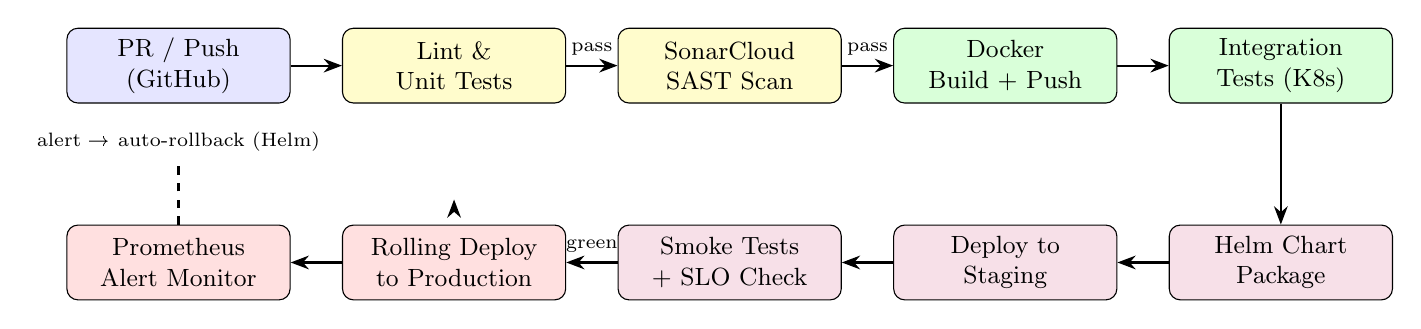
\begin{tikzpicture}[every node/.style={font=\small}]

    %% Stage nodes — horizontal
    \node[block, text width=2.6cm]  (pr)    at ( 0,    0) {PR / Push\\(GitHub)};
    \node[blockY, text width=2.6cm] (lint)  at ( 3.5,  0) {Lint \&\\Unit Tests};
    \node[blockY, text width=2.6cm] (sonar) at ( 7.0,  0) {SonarCloud\\SAST Scan};
    \node[blockG, text width=2.6cm] (build) at (10.5,  0) {Docker\\Build + Push};
    \node[blockG, text width=2.6cm] (integ) at (14.0,  0) {Integration\\Tests (K8s)};

    \draw[arrow] (pr) -- (lint);
    \draw[arrow] (lint) -- node[above, font=\scriptsize]{pass} (sonar);
    \draw[arrow] (sonar) -- node[above, font=\scriptsize]{pass} (build);
    \draw[arrow] (build) -- (integ);

    %% Second row
    \node[blockP, text width=2.6cm] (helm)  at (14.0, -2.5) {Helm Chart\\Package};
    \node[blockP, text width=2.6cm] (stag)  at (10.5, -2.5) {Deploy to\\Staging};
    \node[blockP, text width=2.6cm] (smoke) at ( 7.0, -2.5) {Smoke Tests\\+ SLO Check};
    \node[blockR, text width=2.6cm] (prod)  at ( 3.5, -2.5) {Rolling Deploy\\to Production};
    \node[blockR, text width=2.6cm] (mon2)  at ( 0,   -2.5) {Prometheus\\Alert Monitor};

    \draw[arrow] (integ.south) -- (helm.north);
    \draw[arrow] (helm)  -- (stag);
    \draw[arrow] (stag)  -- (smoke);
    \draw[arrow] (smoke) -- node[above, font=\scriptsize]{green} (prod);
    \draw[arrow] (prod)  -- (mon2);

    %% Rollback path
    \draw[dasharrow] (mon2.north) -- ++(0, 0.8) -- ++(0.0, 0)
         node[above, font=\scriptsize]{alert → auto-rollback (Helm)} (3.5, -1.7);

  \end{tikzpicture}
  \caption{CI/CD Pipeline: from pull request to production rolling deployment.}
  \label{fig:cicd}
\end{figure}

\subsection{Pipeline Stage Specifications}

\subsubsection{Lint and Unit Tests}

Each microservice's GitHub Actions workflow executes \texttt{pylint} (Python code style),
\texttt{mypy} (static type checking), and \texttt{pytest} (unit tests with $\geq$80\%
line coverage requirement). Test failures block the pipeline at this stage, preventing
untested code from reaching the container build phase.

\subsubsection{SAST Scan with SonarCloud}

The static application security testing (SAST) stage runs a SonarCloud scan against all
microservice codebases. This stage is consistent with the DevSecOps posture required for
handling personal behavioral data under GDPR: any new code introducing a critical
security vulnerability (CWE classification) blocks the PR merge. The SonarCloud quality
gate is configured with a coverage delta threshold of $\geq$75\% on new code, a maximum
of zero critical bugs, and zero security hotspots in the \textit{to review} state.

\subsubsection{Docker Multi-Stage Build}

Each microservice uses a two-stage Dockerfile: (i)~a \textit{builder} stage based on
\texttt{python:3.11-slim} that installs dependencies and runs tests; (ii)~a
\textit{runtime} stage that copies only the compiled application artifact, reducing the
final image size by approximately 60\% relative to a single-stage build. Images are
pushed to Amazon ECR with both a version tag (\texttt{v1.2.3}) and a SHA tag
(\texttt{sha-abc1234}) for immutable deployment references.

\subsubsection{Integration Tests on Kubernetes}

Integration tests are executed against a minimal Kubernetes namespace (\texttt{ns:test})
spun up in the CI pipeline using the same Helm chart as production, but with reduced
replica counts. Tests validate: (i)~the Kafka producer-consumer roundtrip latency;
(ii)~the InfluxDB write-read roundtrip; and (iii)~the Inference Microservice HTTP
response on a known test payload.

\subsubsection{Staging Deployment and Smoke Tests}

The Helm chart is deployed to the \texttt{ns:staging} namespace with production
configuration values. Smoke tests execute the full telemetry ingestion path with a
synthetic device UUID, verifying end-to-end data flow from API Gateway through InfluxDB
to Risk Score output. SLO compliance is checked against the P99 latency target.

\subsubsection{Production Rolling Deployment and Auto-Rollback}

Production deployments use Kubernetes rolling update strategy (\texttt{maxUnavailable:
0}, \texttt{maxSurge: 1}) to ensure zero-downtime releases. If Prometheus alerts detect
an error rate exceeding 1\% within 5~minutes of a new deployment, the GitHub Actions
workflow automatically executes \texttt{helm rollback} to the previous chart revision.

%% ============================================================
\section{Observability and Monitoring Architecture}
%% ============================================================

\subsection{Observability Pillars}

The observability architecture is structured around the three industry-standard pillars:
metrics (Prometheus), logs (structured JSON to CloudWatch), and traces (Zipkin via
Istio). Together, these pillars provide full operational visibility into the platform's
health and performance at all times.

\subsection{Prometheus Metrics per Microservice}

Each FastAPI microservice exposes a \texttt{/metrics} endpoint in Prometheus format via
the \texttt{prometheus\_fastapi\_instrumentator} library. Table~\ref{tab:metrics}
specifies the custom application metrics defined for each service.

\begin{table}[H]
  \centering
  \caption{Custom Prometheus Metrics per Microservice}
  \label{tab:metrics}
  \begin{tabularx}{\textwidth}{p{4cm} p{4cm} X}
    \toprule
    \textbf{Microservice} & \textbf{Metric Name} & \textbf{Description} \\
    \midrule
    Rule Engine & \texttt{cvs\_rule\_violations\_total} &
      Counter: total 20-20-20 threshold breaches detected \\
    Normalizer & \texttt{cvs\_normalization\_latency\_ms} &
      Histogram: per-batch normalization processing time \\
    Anonymizer & \texttt{cvs\_dp\_noise\_applied\_total} &
      Counter: total records with Laplace noise applied \\
    Inference Svc & \texttt{cvs\_risk\_score\_value} &
      Gauge: distribution of CVS Risk Scores in the last 5 min \\
    Inference Svc & \texttt{cvs\_model\_version} &
      Gauge: currently loaded model artifact version \\
    Alert Dispatcher & \texttt{cvs\_alerts\_dispatched\_total} &
      Counter: total FCM push notifications dispatched \\
    \bottomrule
  \end{tabularx}
\end{table}

\subsection{Grafana Dashboard Design}

Three Grafana dashboards are provisioned in the \texttt{ns: data \& ml} namespace:

\begin{enumerate}
  \item \textbf{Platform Operations Dashboard:} Kafka consumer lag per partition,
        API Gateway request rate and error rate, HPA replica counts per microservice,
        InfluxDB write throughput, and P99 ingestion latency. This dashboard is the
        primary on-call tool for the IT/DevOps Administrator.
  \item \textbf{Organizational Health Dashboard:} CVS Risk Score distribution across
        the organizational unit (histogram), percentage of high-risk devices by
        department (time series), break compliance trends (weekly), and alert
        acknowledgment rate. This dashboard is the primary interface for the
        Organizational Health Officer.
  \item \textbf{ML Model Performance Dashboard:} Model artifact version timeline,
        risk score statistical distribution drift (KL-divergence over rolling 7-day
        windows), feature importance evolution across model versions, and inference
        latency P50/P95/P99.
\end{enumerate}

\subsection{Distributed Tracing}

The Istio service mesh instruments all inter-pod HTTP/gRPC calls with Zipkin-compatible
distributed tracing headers. Each telemetry ingestion request generates a trace spanning
all five processing hops: Kong Gateway → Kafka Producer → Normalizer → Anonymizer →
InfluxDB Writer. Trace sampling is set to 1\% in production (to limit overhead) and
100\% in staging. The trace data is exported to a Tempo backend and visualized in Grafana
through the TraceQL query interface, allowing the identification of latency outliers
and slow spans within the processing pipeline.

%% ============================================================
\section{Data Governance and Compliance Framework}
%% ============================================================

\subsection{GDPR Article-by-Article Compliance Mapping}

Table~\ref{tab:gdpr} maps the specific GDPR articles applicable to the platform's
data collection and processing activities to the concrete architectural mechanisms that
ensure compliance \cite{b12}.

\begin{table}[H]
  \centering
  \caption{GDPR Compliance Mapping}
  \label{tab:gdpr}
  \begin{tabularx}{\textwidth}{p{2cm} p{4cm} X}
    \toprule
    \textbf{GDPR Article} & \textbf{Principle} & \textbf{Architectural Mechanism} \\
    \midrule
    Art.\ 5(1)(a) & Lawfulness, fairness, transparency &
      On-device consent manager displays data collection purpose and scope before
      first telemetry transmission \\
    Art.\ 5(1)(b) & Purpose limitation &
      Telemetry collected exclusively for CVS risk scoring; secondary use
      contractually prohibited in OHO terms-of-service \\
    Art.\ 5(1)(c) & Data minimization &
      Only three sensor signals collected; no camera, microphone, or location data \\
    Art.\ 5(1)(e) & Storage limitation &
      InfluxDB 90-day retention policy automatically prunes older records; S3
      model artifacts expire after 180 days \\
    Art.\ 17 & Right to erasure &
      \texttt{DELETE /v1/users/\{uuid\}} triggers deletion of pseudonymous UUID
      from InfluxDB, Kafka compaction markers, and S3 metadata \\
    Art.\ 25 & Privacy by design &
      Differential privacy applied at ingestion; no raw PII persisted;
      pseudonymous UUID mapping key held by organization only \\
    Art.\ 32 & Security of processing &
      TLS 1.3 in transit; AES-256 at rest; mTLS pod-to-pod; SQLCipher on device \\
    \bottomrule
  \end{tabularx}
\end{table}

\subsection{Data Lifecycle and Lineage}

Figure~\ref{fig:lifecycle} illustrates the complete data lifecycle from collection
to deletion, showing data transformations and access controls at each stage.

\begin{figure}[H]
  \centering
  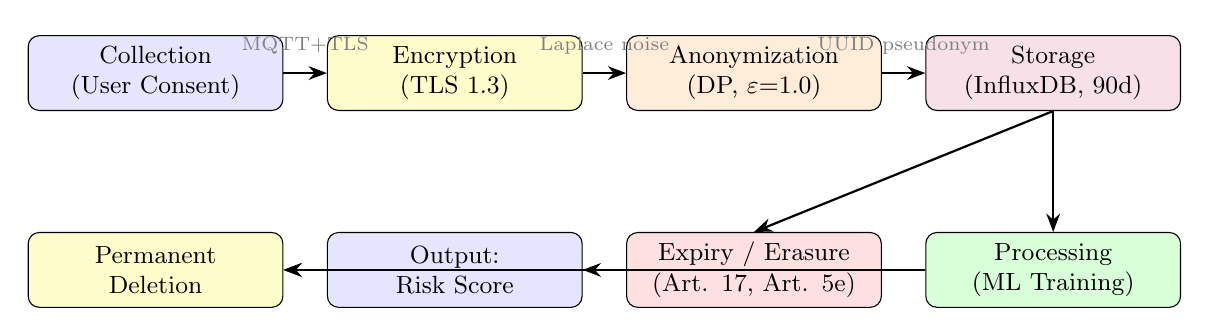
\begin{tikzpicture}[every node/.style={font=\small}]

    %% Lifecycle nodes
    \node[block, text width=3.0cm]  (col)  at (0,    0) {Collection\\(User Consent)};
    \node[blockY, text width=3.0cm] (enc)  at (3.8,  0) {Encryption\\(TLS 1.3)};
    \node[blockO, text width=3.0cm] (anon) at (7.6,  0) {Anonymization\\(DP, $\varepsilon$=1.0)};
    \node[blockP, text width=3.0cm] (stor) at (11.4, 0) {Storage\\(InfluxDB, 90d)};
    \node[blockG, text width=3.0cm] (proc) at (11.4,-2.5){Processing\\(ML Training)};
    \node[blockR, text width=3.0cm] (exp)  at (7.6, -2.5) {Expiry / Erasure\\(Art. 17, Art. 5e)};
    \node[block, text width=3.0cm]  (out)  at (3.8, -2.5) {Output:\\Risk Score};
    \node[blockY, text width=3.0cm] (del)  at (0,   -2.5) {Permanent\\Deletion};

    \draw[arrow] (col) -- (enc);
    \draw[arrow] (enc) -- (anon);
    \draw[arrow] (anon) -- (stor);
    \draw[arrow] (stor) -- (proc);
    \draw[arrow] (stor.south) -- (exp.north);
    \draw[arrow] (proc) -- (out);
    \draw[arrow] (exp) -- (del);
    \draw[arrow] (out) -- (del);

    %% Labels
    \node[font=\scriptsize, text=gray] at (1.9,  0.35) {MQTT+TLS};
    \node[font=\scriptsize, text=gray] at (5.7,  0.35) {Laplace noise};
    \node[font=\scriptsize, text=gray] at (9.5,  0.35) {UUID pseudonym};

  \end{tikzpicture}
  \caption{Data Lifecycle Diagram: from collection to permanent deletion.}
  \label{fig:lifecycle}
\end{figure}

\subsection{Consent Management Flow}

On first application launch, the mobile agent presents the user with a consent dialog
that explicitly describes: (i)~the three sensor signals to be collected; (ii)~the
5-minute micro-batch transmission interval; (iii)~the organizational unit that will
receive anonymized risk dashboard data; (iv)~the 90-day retention period; and (v)~the
right to withdraw consent at any time via the \texttt{DELETE /v1/users/\{uuid\}}
endpoint. User consent is recorded as a SHA-256 hash of the consent document version
and timestamp, stored in the \texttt{consent\_hash} field of each Avro micro-batch.
This hash provides an immutable audit trail demonstrating that each telemetry record
was collected under valid consent, supporting GDPR Article~7 accountability requirements.

%% ============================================================
\section{Architecture Decision Records (ADRs)}
%% ============================================================

This section documents five principal architectural decisions as formal ADRs, following
the lightweight Nygard template \cite{b27}: Title, Status, Context, Decision, Consequences.

\subsection{ADR-001: Apache Kafka as the Central Messaging Backbone}

\textbf{Status:} Accepted. \quad \textbf{Date:} 2026-03-01.

\textbf{Context:} The platform must ingest continuous telemetry micro-batches from
tens of thousands of mobile devices per organizational tenant. Peak hours generate
burst loads that would saturate a synchronous HTTP backend. The Rule Engine, Normalizer,
and Anonymizer must scale independently.

\textbf{Decision:} Apache Kafka 3.6 is adopted as the event streaming backbone.
Kafka decouples producers from consumers, supports exactly-once semantics, and scales
to billions of messages per day with sub-millisecond latency \cite{b10}. A 3-broker
replica configuration provides partition-level fault tolerance. AWS MSK (Managed
Streaming for Kafka) is used in production to reduce operational burden.

\textbf{Consequences — Positive:} Independent consumer scalability; event replay
for debugging; exactly-once delivery guarantee.
\textbf{Consequences — Negative:} Operational complexity of broker cluster;
KRaft quorum configuration required.

\subsection{ADR-002: InfluxDB over TimescaleDB for Time-Series Persistence}

\textbf{Status:} Accepted. \quad \textbf{Date:} 2026-03-01.

\textbf{Context:} The platform must persist high-throughput continuous sensor readings
with efficient time-range query capability for ML feature engineering.

\textbf{Decision:} InfluxDB 2.7 OSS is selected. It exhibits superior performance
for write-heavy IoT metric workloads and provides native 90-day data retention policy
support, simplifying GDPR Article~5(1)(e) compliance \cite{b7}.

\textbf{Consequences — Positive:} Lower write amplification; Flux query language
optimized for time-series aggregations; native Grafana data source plugin.
\textbf{Consequences — Negative:} Weaker SQL ecosystem; migration to TimescaleDB
recommended if JOIN operations with relational metadata become a primary pattern.

\subsection{ADR-003: XGBoost Gradient Boosted Trees for CVS Risk Scoring}

\textbf{Status:} Accepted. \quad \textbf{Date:} 2026-03-05.

\textbf{Context:} The Inference Microservice must produce CVS Risk Scores with
sub-100~ms latency without GPU hardware, using 9 engineered features.

\textbf{Decision:} XGBoost~2.0 Gradient Boosted Trees are adopted. Tree ensembles
outperform neural networks on small-feature tabular datasets \cite{b19}, and provide
interpretable feature importances. Inference requires no GPU and completes in
$<$10~ms on CPU-optimized pods.

\textbf{Consequences — Positive:} Fast inference; interpretable outputs; no GPU cost.
\textbf{Consequences — Negative:} Tree models may underfit complex temporal patterns;
LSTM sequential models are designated as a future evaluation target.

\subsection{ADR-004: Differential Privacy ($\varepsilon = 1.0$) at the Anonymizer Layer}

\textbf{Status:} Accepted. \quad \textbf{Date:} 2026-03-05.

\textbf{Context:} The platform collects behavioral data classified as personal data
under GDPR. Raw sensor readings transmitted to the cloud create re-identification risk.

\textbf{Decision:} The Anonymizer Microservice applies Laplace-distributed noise with
privacy budget $\varepsilon = 1.0$. This configuration satisfies GDPR compliance while
maintaining utility loss below 5 percentage points \cite{b11,b23}. Device identifiers
are replaced by pseudonymous UUIDs at first consent.

\textbf{Consequences — Positive:} Mathematical privacy guarantee; GDPR compliance;
enables population-level model training without raw data exposure.
\textbf{Consequences — Negative:} Introduces noise in individual readings;
$\varepsilon$ must be re-tuned per deployment jurisdiction.

\subsection{ADR-005: Kong API Gateway for Authentication and Rate Control}

\textbf{Status:} Accepted. \quad \textbf{Date:} 2026-03-08.

\textbf{Context:} All inbound telemetry requests must be authenticated, rate-limited
to prevent DDoS from compromised devices, and provide a single auditable entry point.

\textbf{Decision:} Kong Gateway 3.x enforces JWT/OAuth2 validation using tokens signed
by Keycloak. Microservices validate signatures locally (stateless JWT pattern) without
contacting the IdP on every request \cite{b9}. mTLS between pods is enforced by Istio.

\textbf{Consequences — Positive:} Centralized authentication; rate limiting; observability.
\textbf{Consequences — Negative:} Kong is a potential single point of failure; mitigated
by deploying 2+ Kong replicas behind the Kubernetes load balancer.

%% ============================================================
\section{Quality Attributes and Service Level Objectives}
%% ============================================================

\subsection{Quality Attribute Scenarios}

Following the Architecture Tradeoff Analysis Method (ATAM), four primary quality
attributes are defined with measurable scenarios and target SLOs, as shown in
Table~\ref{tab:slos}.

\begin{table}[H]
  \centering
  \caption{Quality Attribute Scenarios and Target SLOs}
  \label{tab:slos}
  \begin{tabularx}{\textwidth}{p{2.5cm} p{4.5cm} p{3cm} p{3.5cm}}
    \toprule
    \textbf{Quality Attr.} & \textbf{Scenario} & \textbf{Target SLO} &
    \textbf{Architectural Mechanism} \\
    \midrule
    Availability & System continues processing telemetry during a single Kafka broker
      failure & $\geq 99.5\%$ uptime/month & 3-replica Kafka; K8s liveness probes; HPA \\
    \addlinespace
    Scalability & System sustains 10,000 concurrent device connections with
      $<$500~ms ingestion latency & P99 latency $\leq 500$~ms under 10k producers &
      Kafka partitioning; stateless microservices; HPA \\
    \addlinespace
    Security & No raw PII persisted; all inter-service communication encrypted &
      Zero raw PII in InfluxDB; 100\% mTLS inter-pod &
      Anonymizer DP; Istio mTLS; InfluxDB AES-256 at rest \\
    \addlinespace
    ML Accuracy & CVS Risk Score correctly classifies high-risk users &
      F1-score $\geq 0.75$; AUC-ROC $\geq 0.80$ &
      XGBoost; 5-fold CV; 9-feature engineering \\
    \addlinespace
    ML Inference & Inference Microservice responds within latency bound &
      P99 inference latency $\leq 100$~ms &
      XGBoost CPU inference; HPA; stale model cache \\
    \bottomrule
  \end{tabularx}
\end{table}

\subsection{Scalability Analysis}

The platform's horizontal scalability stems from three compounding mechanisms.
First, Kafka's partitioned log allows consumer throughput to scale linearly with
partition count: doubling partitions from 12 to 24 approximately doubles parallel
consumer capacity without producer code changes \cite{b10}. Second, the Kubernetes
HPA adds processing pods when CPU utilization exceeds the configured threshold,
providing elastic burst capacity aligned with empirical findings from healthcare
Kubernetes deployments \cite{b20}. Third, InfluxDB's internal compaction and sharding
maintain query performance as data volume grows, with documented advantages for
high-cardinality IoT write workloads \cite{b7}.

A theoretical back-of-envelope capacity estimate: at 10,000 concurrent devices, each
transmitting one Avro micro-batch (approximately 1.2~KB binary) every 5~minutes,
the aggregate ingestion throughput is $10{,}000 \times 1200 / 300 \approx 40$~KB/s,
well within Kafka's documented throughput envelope of hundreds of MB/s per broker.

\subsection{Privacy Compliance Analysis}

GDPR compliance is achieved through a defense-in-depth privacy stack:
(i)~on-device consent management (Art.~7); (ii)~TLS~1.3 in transit (Art.~32);
(iii)~Laplace differential privacy noise at the Anonymizer layer (Art.~25, 32);
(iv)~pseudonymous UUID mapping (Art.~4(5)); and (v)~automated data retention expiry
at 90 days (Art.~5(1)(e)). This layered approach is consistent with the principle
that combining differential privacy with secure aggregation creates sufficient security
to satisfy GDPR legal requirements in healthcare data contexts \cite{b11,b13,b23}.

%% ============================================================
\section{Economic Impact Analysis}
%% ============================================================

\subsection{Organizational Cost-Benefit Model}

The economic case for deploying the CVS platform at the organizational level can be
modeled around the productivity recovery value generated by reduced CVS incidence.
Based on the Deloitte/AOA report \cite{b16}, an average desk worker affected by
unmanaged CVS loses 18.6\% of productive output, equivalent to approximately 7.4
hours per working week. For an organization with $N$ knowledge workers and an average
annual labor cost of $C$ USD per employee, the annual productivity loss attributable
to CVS is approximated as:

\begin{equation}
  L_{\text{CVS}} = N \times C \times 0.186 \times p_{\text{CVS}}
  \label{eq:loss}
\end{equation}

where $p_{\text{CVS}} = 0.69$ is the global CVS prevalence rate \cite{b15}.

For a representative Colombian enterprise with 1,000 knowledge workers and an average
annual labor cost of \$18,000 USD per employee (consistent with median professional
salaries in Bogotá's technology sector), this yields:

\begin{equation}
  L_{\text{CVS}} = 1{,}000 \times 18{,}000 \times 0.186 \times 0.69
  \approx \$2.31\text{ million USD/year}
  \label{eq:colombia}
\end{equation}

Conservative estimates suggest that a well-implemented proactive CVS mitigation program
can reduce CVS prevalence among enrolled workers by 30--40\% through timely break
reminders and ergonomic interventions. Applying a conservative 30\% reduction factor:

\begin{equation}
  \text{Annual Productivity Recovery} \approx \$2.31M \times 0.30 \approx \$693{,}000
  \label{eq:recovery}
\end{equation}

\subsection{Platform Operating Cost Estimate}

Table~\ref{tab:costs} estimates the monthly cloud infrastructure cost for the prototype
deployment configuration supporting 1,000 concurrent devices on AWS EKS.

\begin{table}[H]
  \centering
  \caption{Estimated Monthly Cloud Infrastructure Cost (AWS, 1k Devices)}
  \label{tab:costs}
  \begin{tabularx}{\textwidth}{p{4.5cm} p{3cm} X}
    \toprule
    \textbf{Component} & \textbf{Estimated Cost/Month} & \textbf{Notes} \\
    \midrule
    EKS Cluster (3 node pools) & \$220 & t3.medium instances, 6 nodes total \\
    AWS MSK (Kafka, 3 brokers) & \$180 & kafka.t3.small, 50 GB storage/broker \\
    InfluxDB (StatefulSet, gp3) & \$45  & 100 GB gp3 SSD persistent volume \\
    S3 (model artifacts)         & \$5   & $<$10 GB model store \\
    Kong Gateway (ELB)           & \$30  & Application Load Balancer \\
    Prometheus + Grafana          & \$20  & Single-replica; shared node \\
    GitHub Actions (CI/CD)        & \$15  & Paid minutes for private repo \\
    \midrule
    \textbf{Total}               & \textbf{\$515/month} & (\$6,180/year) \\
    \bottomrule
  \end{tabularx}
\end{table}

The annual ROI for the 1,000-employee scenario is therefore approximately:

\begin{equation}
  \text{ROI} = \frac{\$693{,}000 - \$6{,}180}{\$6{,}180} \approx 111\times
  \label{eq:roi}
\end{equation}

This result indicates a strongly positive economic case for enterprise deployment,
with infrastructure costs representing less than 1\% of the projected productivity
recovery value. It is important to note that these estimates carry uncertainty due
to the assumptions on intervention effectiveness and the Colombian salary baseline
used; the third-phase evaluation will refine these estimates based on empirical
measurement of the system's actual break-compliance improvement rates.

%% ============================================================
\section{Risk Analysis and Mitigation}
%% ============================================================

Table~\ref{tab:risks} identifies the principal technical and operational risks
associated with the prototype architecture, their probability and impact assessment,
and the mitigation strategy implemented at the architectural level.

\begin{table}[H]
  \centering
  \caption{Risk Analysis Matrix}
  \label{tab:risks}
  \begin{tabularx}{\textwidth}{p{3.5cm} p{1.3cm} p{1.3cm} p{4cm} X}
    \toprule
    \textbf{Risk} & \textbf{Prob.} & \textbf{Impact} & \textbf{Mitigation Strategy} &
    \textbf{Residual Risk} \\
    \midrule
    Kafka broker failure & Medium & High &
      3-replica cluster; auto-recovery via K8s liveness probes; MSK managed failover &
      Low: P99 TTR $\leq$30s expected \\
    \addlinespace
    InfluxDB disk saturation & Low & High &
      90-day retention policy; Grafana alert at 70\% disk utilization; gp3 auto-scaling &
      Very low \\
    \addlinespace
    ML model drift (concept drift) & Medium & Medium &
      Rolling 7-day KL-divergence monitoring on risk score distribution; automatic
      nightly retraining CronJob &
      Medium: requires labeled ground truth \\
    \addlinespace
    \texttt{UsageStatsManager} permission denial & Medium & Medium &
      Alternative foreground activity detection via \texttt{ActivityManager};
      documented as fallback path &
      Low: degrades screen time accuracy only \\
    \addlinespace
    GDPR right-to-erasure latency & Low & High &
      \texttt{DELETE} endpoint triggers async deletion across InfluxDB, Kafka compact,
      S3; completion SLO of 30 days per GDPR Art. 12 &
      Low: GDPR allows 30-day window \\
    \addlinespace
    Kong Gateway DDoS from compromised devices & Low & High &
      Per-device rate limiting (100 req/min); IP-based Kong rate plugin; circuit breaker
      (ADR-001) &
      Low \\
    \addlinespace
    Synthetic label misalignment with clinical ground truth & High & Medium &
      Labels derived from clinical thresholds \cite{b2}; third-phase evaluation will
      compare against optometrist-validated survey data &
      Medium: acknowledged limitation \\
    \bottomrule
  \end{tabularx}
\end{table}

%% ============================================================
\section{Evaluation Methodology for Phase Three}
%% ============================================================

The third phase of this project will conduct an empirical evaluation of the deployed
prototype against the SLOs defined in Table~\ref{tab:slos}. The following experimental
designs are specified.

\subsection{Load Testing (Scalability SLO)}

An Apache JMeter load test will simulate 10,000 concurrent MQTT producers transmitting
micro-batches at 5-minute intervals. The test runs for 60~minutes to allow HPA
stabilization. Metrics collected: Kafka consumer lag per partition, P50/P95/P99 ingestion
latency (Prometheus), and HPA scale-out event count. The Scalability SLO passes if P99
latency remains at or below 500~ms throughout the sustained load period.

\subsection{Fault Injection (Availability SLO)}

A controlled fault injection experiment terminates one Kafka broker pod with
\texttt{kubectl delete pod} during active load at the 20-minute mark of the load test.
The time-to-recovery (TTR) for all affected partitions is measured from the deletion
event to the restoration of zero consumer lag. The Availability SLO passes if TTR
$\leq 30$~seconds, consistent with Kafka's documented controller-election behavior
\cite{b10}.

\subsection{ML Model Evaluation (ML Accuracy SLO)}

The XGBoost model will be trained on a synthetic behavioral dataset of 50,000
user-day records, calibrated to the clinical thresholds of Sheppard and Wolffsohn
\cite{b2}. The held-out test set (20\%) will be evaluated for: F1-score (macro average),
AUC-ROC, Precision, and Recall. Feature importance analysis will verify that
\texttt{max\_cont\_session\_min} and \texttt{break\_compliance\_score} rank among the
top three contributors, as expected from the clinical literature.

\subsection{Privacy Audit (Security SLO)}

An automated assertion suite will verify that zero raw PII fields appear in any
InfluxDB write-path data. A Kolmogorov-Smirnov test will verify that the Laplace
noise injection preserves the original sensor distributions within a threshold of
$p > 0.05$, confirming that the DP mechanism does not distort statistical utility
beyond acceptable bounds.

\subsection{Inference Latency Benchmark (Inference SLO)}

The Inference Microservice will be benchmarked under a sustained request rate of
1,000 risk score requests per minute using \texttt{locust.io}. The benchmark runs
for 10~minutes and records P50, P95, and P99 inference latency. The Inference SLO
passes if P99 latency remains at or below 100~ms.

%% ============================================================
\section{Discussion}
%% ============================================================

\textbf{From reactive to proactive.} The ML inference pipeline computes a population-
calibrated CVS Risk Score reflecting the interaction of multiple behavioral factors,
enabling preemptive intervention before symptomatic onset---a capability absent from all
existing commercial tools reviewed in the related work.

\textbf{From edge silos to organizational intelligence.} The cloud-native architecture
aggregates anonymized behavioral signals across entire organizational units, enabling
Health Officers to identify high-risk departments or usage patterns invisible to any
individual device's local analytics. This aligns with the TOGAF Business Architecture
objective of providing actionable visibility into the ``digital wear'' of human capital.

\textbf{From camera-based to non-invasive proxy sensing.} The exclusive reliance on
ambient light, proximity, and interaction time avoids the documented privacy rejection
associated with continuous camera-based monitoring \cite{b4}. The precision trade-off
is compensated by operating on 30-day behavioral windows and population-level baselines
rather than instantaneous physiological readings.

One acknowledged limitation is the dependency on Android's \texttt{UsageStatsManager}
API, which requires a special system permission not uniformly grantable in all enterprise
MDM configurations. The alternative foreground activity detection path described in the
risk analysis (Table~\ref{tab:risks}) provides a fallback at reduced accuracy.
Additionally, the synthetic label construction introduces potential misalignment with
ground-truth clinical assessment; this will be partially addressed in the third phase
by comparing model predictions against optometrist survey responses from a volunteer
participant group.

%% ============================================================
\section{Conclusions and Future Work}
%% ============================================================

This article has presented the complete general architecture and prototype design for
a distributed cloud-native platform for the proactive mitigation of Computer Vision
Syndrome through behavioral telemetry analytics. The principal contributions are:

\begin{enumerate}
  \item A \textbf{formally specified four-layer architecture} documented through five
        complementary IEEE/ISO~42010-aligned architectural views: context, component,
        data-flow, deployment, and security.
  \item A \textbf{TOGAF ADM-aligned enterprise architecture} view mapping the four
        TOGAF domains (Business, Data, Application, Technology) to the platform's
        structural components, supporting the organizational governance objectives of
        the course.
  \item A \textbf{prototype technology stack} with technically justified selections:
        Apache Kafka for event streaming, InfluxDB for time-series persistence,
        XGBoost for CVS Risk Score inference, Kubernetes/Helm for orchestration, and
        Kong/Istio for security enforcement.
  \item \textbf{Five Architecture Decision Records (ADRs)} formalizing the most
        consequential design choices, including the differential privacy configuration,
        the ML model selection, and the API Gateway strategy.
  \item \textbf{Four applied microservices design patterns} (Database-per-Service,
        Event Sourcing, CQRS, Circuit Breaker) with concrete realizations in the
        prototype, increasing resilience, consistency, and operational observability.
  \item A \textbf{CI/CD and observability architecture} covering the complete DevSecOps
        pipeline from pull request to production deployment with auto-rollback.
  \item A \textbf{GDPR-compliant data governance framework} with Article-by-Article
        compliance mapping and a formal data lifecycle diagram.
  \item \textbf{Five measurable SLOs} (availability $\geq 99.5\%$; P99 latency
        $\leq 500$~ms under 10k producers; zero raw PII in persistence; F1 $\geq 0.75$;
        inference P99 $\leq 100$~ms) with specified evaluation methodology for Phase~3.
  \item An \textbf{economic impact analysis} demonstrating a theoretical ROI of
        approximately $111\times$ for a 1,000-employee Colombian enterprise.
\end{enumerate}

The third phase will focus on: (i)~deploying the Helm chart to a managed EKS cluster;
(ii)~executing the load testing, fault injection, and privacy audit experiments;
(iii)~training the XGBoost model on a synthetic behavioral dataset calibrated to
the clinical thresholds of Sheppard and Wolffsohn \cite{b2}; and (iv)~reporting
quantitative quality attribute measurements against all defined SLOs. The long-term
vision is a platform that enables organizations to treat CVS not as an individual
productivity nuisance but as a measurable, monitorable, and systematically reducible
occupational health risk at the enterprise scale.

%% ============================================================
%%  BIBLIOGRAPHY
%% ============================================================
\begin{thebibliography}{00}

\bibitem{b1}
R. A. Elhai, J. D. Elhai, and B. J. Hall,
``Future directions in the study of technology addiction,''
\textit{Addictive Behaviors}, vol. 112, 2021.

\bibitem{b2}
A. L. Sheppard and J. S. Wolffsohn,
``Digital eye strain: prevalence, measurement and amelioration,''
\textit{BMJ Open Ophthalmology}, vol. 3, no. 1, p. e000146, 2018.

\bibitem{b3}
C. Blehm, S. Vishnu, A. Khattak, S. Mitra, and R. W. Yee,
``Computer vision syndrome: a review,''
\textit{Survey of Ophthalmology}, vol. 50, no. 3, pp. 253--262, 2005.

\bibitem{b4}
N. D. Lane et al.,
``A survey of mobile phone sensing,''
\textit{IEEE Communications Magazine}, vol. 48, no. 9, pp. 140--150, Sept. 2010.

\bibitem{b5}
A. A. Mutlag, M. K. Abd Ghani, N. Arunkumar, M. A. Mohammed, and O. Mohd,
``Enabling technologies for fog computing in healthcare IoT systems,''
\textit{Future Generation Computer Systems}, vol. 90, pp. 62--78, 2019.

\bibitem{b6}
K. Mahmoud, K. Orsborn, and T. Risch,
``Survey on IoT application architectures,''
\textit{MDPI Sensors}, 2024. [Online].
Available: https://pmc.ncbi.nlm.nih.gov/articles/PMC11360728/

\bibitem{b7}
OctaByte,
``InfluxDB vs TimescaleDB: Which is Better for Time-Series Data?''
Sept. 2025. [Online].
Available: https://blog.octabyte.io/topics/open-source-databases/influxdb-vs-timescaledb/

\bibitem{b8}
S. B. Chauhan and R. N. Gore,
``SMQTT: A Lightweight Clock Synchronization Algorithm for IoT Devices Using MQTT,''
in \textit{Proc. IEEE ISPCS}, London, UK, 2023, pp. 1--6.

\bibitem{b9}
Paradigma Digital,
``Architecture Patterns in Microservices: Security with JWT,'' 2024. [Online].
Available: https://en.paradigmadigital.com/dev/architecture-patterns-microservices-security-jwt/

\bibitem{b10}
Apache Software Foundation,
``Apache Kafka 3.6 Documentation,'' 2024. [Online].
Available: https://kafka.apache.org/documentation/

\bibitem{b11}
B. M. Alotaibi et al.,
``Privacy-Preserving, Regulatory-Grade Real-Time Healthcare AI,''
\textit{American Journal of Technology}, Dec. 2025. [Online].
Available: https://gprjournals.org/journals/index.php/ajt/article/view/459

\bibitem{b12}
European Parliament and Council,
``Regulation (EU) 2016/679 — General Data Protection Regulation (GDPR),'' 2016.

\bibitem{b13}
V. Berneker et al.,
``Federated Machine Learning, Privacy-Enhancing Technologies, and Data Protection Laws
in Medical Research: Scoping Review,''
\textit{J. Med. Internet Res.}, vol. 25, p. e41588, 2023.

\bibitem{b14}
H. Ali et al.,
``Federated Learning in Smart Healthcare: A Comprehensive Review on Privacy, Security,
and Predictive Analytics with IoT Integration,''
\textit{MDPI Electronics}, Dec. 2024.
Available: https://pmc.ncbi.nlm.nih.gov/articles/PMC11728217/

\bibitem{b15}
SmartErgo,
``December 2024: Digital Eye Strain Prevalence and Mitigation Into 2025,'' 2024.
[Online].
Available: https://smartergo.com/december-2024-digital-eye-strain-prevalence-and-mitigation-into-2025/

\bibitem{b16}
American Optometric Association and Deloitte Economics Institute,
``The Impact of Unmanaged Excessive Screen Time in the United States,'' 2023.
[Online]. Available: https://www.aoa.org/AOA/Documents/Eye\%20Deserve\%20More/Cost\%20of\%20Unmanaged\%20Screen\%20Time\%20Report\_FINAL.pdf

\bibitem{b17}
VSP Vision Care and Workplace Intelligence,
``2025 Workplace Vision Health Report,'' 2025. [Online].
Available: https://workplaceintelligence.com/2024-workplace-vision-health/

\bibitem{b18}
J. Talens-Estarelles et al.,
``Digital eye strain symptoms worsen during prolonged digital tasks, associated with
a reduction in productivity,''
\textit{Optometry and Vision Science}, Sept. 2024.

\bibitem{b19}
N. Alshurafa et al.,
``Wearable network for multilevel physical fatigue prediction in manufacturing workers,''
\textit{PNAS Nexus}, vol. 3, no. 10, p. pgae421, 2024.

\bibitem{b20}
V. V. R. Boda and H. Allam,
``Scaling Kubernetes for Healthcare: Real Lessons from the Field,''
\textit{Int. J. Emerg. Res. Eng. Technol.}, vol. 4, no. 3, pp. 27--34, 2023.

\bibitem{b21}
M. Nygard,
``Architecture Decision Records,'' 2011. [Online].
Available: https://cognitect.com/blog/2011/11/15/documenting-architecture-decisions

\bibitem{b22}
J. Chae et al.,
``Visual fatigue prediction using classification model based on physiological responses
of occupants under office lightings,''
\textit{Journal of Building Engineering}, Oct. 2024.

\bibitem{b23}
A. A. Mutlag et al.,
``Privacy preservation for federated learning in healthcare,''
\textit{Patterns (N.Y.)}, vol. 5, no. 7, p. 100974, July 2024.

\bibitem{b24}
The Open Group,
``TOGAF\textsuperscript{\textregistered} Standard, 10th Edition,'' 2022. [Online].
Available: https://www.opengroup.org/togaf

\bibitem{b25}
D. Pal, J. London, A. Aakula, and S. Chitta,
``Implementing TOGAF for Large-Scale Healthcare Systems Integration,''
\textit{IoT and Edge Computing Journal}, 2024.
Available: https://thesciencebrigade.com/iotecj/article/view/464

\bibitem{b26}
X.-K. Yeh,
``Unpacking the Structure of the TOGAF Standard: A Strategic Blueprint for
Enterprise Architects,'' \textit{Medium}, Oct. 2025. [Online].
Available: https://medium.com/@leoyeh.me

\bibitem{b27}
M. Nygard,
``Architecture Decision Records,'' \textit{Cognitect Blog}, 2011. [Online].
Available: https://cognitect.com/blog/2011/11/15/documenting-architecture-decisions

\bibitem{b28}
C. Richardson,
``Microservices Patterns: With Examples in Java,'' 1st ed.
Manning Publications, 2018.

\bibitem{b29}
Atlassian,
``7 Essential Microservices Design Patterns,'' 2024. [Online].
Available: https://www.atlassian.com/microservices/cloud-computing/microservices-design-patterns

\end{thebibliography}

\end{document}